\documentclass[11pt]{article}
%\usepackage[margin=1in]{geometry} 
\usepackage{template}
\usepackage[center]{titlesec}

\titleformat{\section}% command to format the section titles
        [block]% shape/type of title
        {\LARGE\bfseries\centering}% formatting commands applied to both label and title
        {\thesection.}% section number; here set inside an invisible box with a constant width
        {1ex}% separation between number and chapter title; we've already covered this with the box
        {}% additional formatting command for title itself not applied to number
        [
        ]%
        

\usepackage[utf8]{inputenc} % allow utf-8 input
\usepackage[T1]{fontenc}    % use 8-bit T1 fonts
\usepackage{hyperref}       % hyperlinks
\usepackage{url}            % simple URL typesetting
\usepackage{booktabs}       % professional-quality tables
\usepackage{amsfonts}       % blackboard math symbols
\usepackage{nicefrac}       % compact symbols for 1/2, etc.
\usepackage{microtype}      % microtypography
\usepackage{lipsum}
\usepackage[labelfont=bf]{caption}
\usepackage{subcaption}
\usepackage{amsmath,amsthm,amssymb}
\usepackage[english]{babel}
\usepackage{comment}
\usepackage{enumitem}

\usepackage{graphicx}
\graphicspath{ {images/} }

\usepackage{floatrow}
\usepackage{listings}
\usepackage{minted}
\floatsetup[listing]{style=Plaintop}    

\usepackage{float}
\usepackage{texments}
\usestyle{default} %other useful styles are, bw,  borland, vs
\usepackage[dvipsnames]{xcolor}
\usepackage[toc,page]{appendix}
%\usepackage[titletoc]{appendix}
\usepackage{minted}

\usepackage{chngcntr}
\counterwithin{figure}{section}
\counterwithin{table}{section}

%citation
\usepackage{epigraph}

\usepackage{graphicx}

\newcommand{\norm}[1]{\left\lVert#1\right\rVert}

\newcommand{\cac}[1]{{\textcolor{blue}[\textcolor{blue}{\bf{AC: }}{ \textcolor{blue}
              {#1}]}}}
\newcommand{\cgv}[1]{{\textcolor{RedOrange}[\textcolor{RedOrange}{\bf{GV: }}{ \textcolor{RedOrange}
              {#1}]}}}
\newcommand{\mic}[1]{{\textcolor{Green}[\textcolor{Green}{\bf{Micheli: }}{ \textcolor{Green}
              {#1}]}}}
\newcommand{\lf}[1]{{\textcolor{magenta}[\textcolor{magenta}{\bf{L: }}{ \textcolor{magenta}
              {#1}]}}}


%\setcitestyle{square}

%%%%%%%%%%%%%%%%%%%%%%%%%%%%%%%%
%%      Tittle Page Start     %%
%%%%%%%%%%%%%%%%%%%%%%%%%%%%%%%%
\title{IsaNet Library}
\author{
  Alessandro Cudazzo \\
  \texttt{alessandro@cudazzo.com} \\
  %% examples of more authors
   \And
  Giulia Volpi \\
  \texttt{giuliavolpi25.93@gmail.com} \\
  \AND
  Department of Computer Science, University of Pisa, Pisa, Italy
  %% Coauthor \\
  %% Affiliation \\
  %% Address \\
  %% \texttt{email} \\
  %% \And
  %% Coauthor \\
  %% Affiliation \\
  %% Address \\
  %% \texttt{email} \\
  %% \And
  %% Coauthor \\
  %% Affiliation \\
  %% Address \\
  %% \texttt{email} \\
}

%%%%%%%%%%%%%%%%%%%%%%%%%%%%%%%%
%%       Tittle Page End      %%
%%%%%%%%%%%%%%%%%%%%%%%%%%%%%%%%

\begin{document}

\maketitle
\begin{abstract}
In this work, we developed a new Neural Network library in Python, and we called it \textbf{IsaNet Lib}. It provides high and low-level API with an entire module for model selection. First, it was tested on the MONK Datasets (classification tasks) and then on the CUP Dataset (regression task). All the analyses use well-known validation methods (Hold-out, K-fold Cross Validation) to provide a model that can generalize the data.
\end{abstract}

\section{Introduction}
The aims of project \textbf{A} of the Machine Learning (ML) course are to implement an ML model simulator (Neural Network, SVM, ...), understand the hyper-parameters effect on the model and solve a supervised regression learning task by using the CUP dataset provided in the course. For the first aim, we decided to implement a Multi-Layer Perceptron (MLP) model with \textit{back-propagation} (gradient descent), \textit{Classic Momentum} (also known as \textit{Polyak’s heavy ball method}\cite{Polyak1964}), \textit{Nesterov} (introduced in \cite{sutskever2013}), the new \textit{Accelerated Nesterov} (see \cite{nakerst2020gradient}), \textit{L2 regularization}, some \textit{Early Stopping}, and other features. Since the project grows very fast, we decided to develop a neural network library that would allow us to focus on the other aims.  We will explain all the major details of the library in the next session. In order to test and validate our library we used MONK datasets~\cite{Dua:2019} and after that, we moved on to CUP dataset analysis. To determine the best hyper-parameters configuration for the CUP's task we performed a grid search with K-fold cross-validation and the final model was re-trained using hold out as validation method for the early stopping.

The remaining text is structured as follows. In Section~\ref{sec:isanet_lib}, we have illustrated the methods used for all the analysis. The experiments are shown in section Section~\ref{sec:experiment}, Subsections~\ref{sec:monks} and \ref{sec:cup} respectively contain the results of MONK and CUP, while Section~\ref{sec:conclusions} is devoted to conclusions.



\section{Method}
\label{sec:isanet_lib}
In this section, we first present the IsaNet Lib (Sec. \ref{sec:design_code}). Then we describe the Early Stopping and Complexity Control (Sec. \ref{sec:early_stop}), the initialization methods (Sec. \ref{sec:w_init}) used in the experimental phase, and finally, the preprocessing and validation schema (Sec. \ref{sec:preprop} and \ref{sec:validation_schema}).

\subsection{Design and Code Overview}
\label{sec:design_code}
The first step we made was to write a library that would provide us a flexible and modular neural network model. We called it \textbf{IsaNet}. We wrote the library entirely in Python using Numpy as a package for scientific computation. All the main operations of a neural network, as the feed-forward and the back-propagation algorithms, are performed by using matrices, and layers of nodes are stored in a list of matrices where columns are the weights of a single node (the bias is the first element). This implementation allowed us to speed up the computation compared to an object-oriented structure (layers, nodes views as object); this was possible thanks to Numpy that can efficiently perform matrix operation by parallelization under the hood. Numpy uses optimized math routines, written in C or Fortran, for linear algebra operation as \textit{Blas}, \textit{OpenBlas} or \textit{Intel Math Kernel Library (MKL)}~\cite{intel-alt}. IsaNet is composed of low and high-level APIs divided into modules.\\

\noindent\textbf{Modules -  Low Level API}:
\begin{itemize}
    \item \texttt{model.py}: this module implement the main class, \texttt{Mlp}, which stands for Multi-Layer Perceptron. The class allows to add one or multi-layers and specify for each of them: a specific number of nodes, an activation function, the range used for the weights initialization, the value of L2 regularization term. Furthermore, it allows you to associate a specific optimizer used to train the model and provide to the user a fitting and predict methods to perform training and prediction operation. In the fitting method, we can specify the training set, the validation set, the maximum number of epochs, the early stopping technique, the number of elements for a minibatch (the library supports full batch, mini-batch and online) and the verbose mode.
    
    \item \texttt{optimizer.py}: this module contains the \texttt{SGD} class, which implements the Stochastic Gradient Descent with mean squared error as loss function and different types of momentum: Classic (CM) , Nesterov (NM) and the new Accelerated Nesterov (ANM) (see \cite{nakerst2020gradient}). In the Appendix \ref{appendix:momentum_comp}, there are some comparisons between the various momentum. Hence, the available hyperparameters are $\eta$ for the learning rate, $\alpha$  for the CM, True/False for the NM, and $\sigma$ for the ANM. Besides, this module provides some Early Stopping to use in the fitting phase. In the \texttt{SGD} we can check if there are no improvements in optimizations (training error), and with the \texttt{EarlyStopping} class provided by the module, we can detect cases of overfitting. For both, we can specify a certain threshold and a maximum number of epochs for which the increase or decrease must occur. Further details on overfitting handling are left in Sec.~\ref{sec:early_stop}.
    
    \item \texttt{activation.py}: this module implements Sigmoid, Identity, Tanh, and Relu activation functions, while \texttt{metrics.py} provide functions for MSE (Mean Square Error), MEE (Mean Euclidean Error), and Accuracy.
\end{itemize}

\noindent\textbf{Modules -  High Level API}:
\begin{itemize}
    \item \texttt{neural\_network.py}: this module provides two main classes, \texttt{MLPRegressor} and \texttt{MLPClassifier}, respectively, a Multi-layer Perceptron Regressor and a Multi-layer Perceptron Classifier. Both classes simplify the creation of an MLP model by specifying the hyper-parameters, as constructor parameters of the class, besides
    %LORE
    %, they provide 
    the classic fitting and prediction operations. All hyper-parameters provided by low level APIs are present for these classes.
    
    \item \texttt{model\_selection.py}: composed of two classes, \texttt{Kfold} and \texttt{GridSearchCV}. One provides the k-folds cross-validation method, and the other implements an exhaustive search on a subset of hyperparameters space called Grid Search.

\end{itemize}
Some examples, showing the use of APIs, have been added in Appendix \ref{appendix:code_example}, and the library is distributed open on GitHub with the related documentation at \href{https://github.com/alessandrocuda/IsaNetNN/}{https://github.com/alessandrocuda/IsaNetNN/}. 

\subsection{Early Stopping and Complexity Control}
\label{sec:early_stop}

\begin{figure}[h]
    \centering
    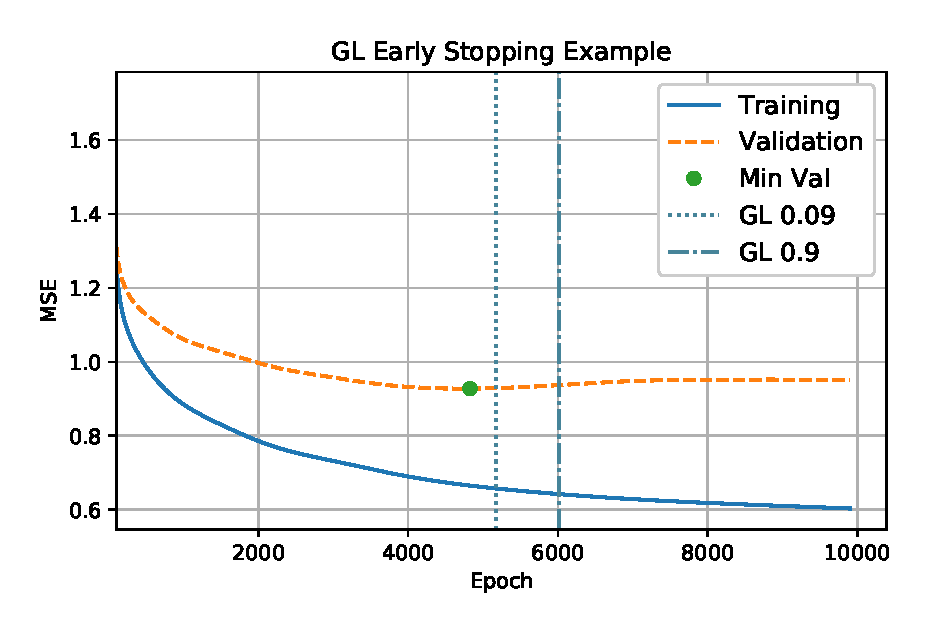
\includegraphics[scale = 0.65]{Images/early_stop.eps}
    \caption{From the generalization error we can see that the model goes into overfitting but minimum of generalization ($MSE = 0.9275$) is reached at 4826 epochs. We can obtain different stop points changing the $\varepsilon_{GL}$ value (suppose $s_{UP}=200$ epochs ): with $\varepsilon_{GL} = 0.09$ the stop point is at 5170 with Validation $MSE = 0.9283$ and with $\varepsilon_{GL} = 0.9$ the stop point is at 6018 with Validation $MSE = 0.9371$. With no early stopping, the fitting will end at the max number of epochs (10000) with $0.9514$ as generalization error.}
    \label{fig:early_stop_example}
\end{figure}
When training an MLP, we can use the validation error to detect overfitting and underfitting. We are generally interested in obtaining the minimum error of generalization and avoiding overfitting. In the ideal case, we expect that the validation curve will show a smooth increase when overfitting occurs, but in reality, this is not always true. In fact, a validation curve may have more local minima, this is well illustrated in \cite{Prechelt2012}, and many methods are proposed in order to handle this problem. Two of them have been implemented and used, as can be seen in Section \ref{sec:experiment}, devoted to experiments. They are: $GL$ (stops as soon as the generalization loss exceeds a certain threshold) and $UP$ (stops when the generalization error increased in \textit{s} successive epochs). From now on, we'll refer to $\varepsilon_{GL}$ as the threshold used in the $GL$ method and to $s_{UP}$ as the max number of epochs in $UP$ method. An example, applied on CUP dataset, is shown in Fig.~\ref{fig:early_stop_example}.

Of course, in addition to the classic early stopping, in the experimental phase we used the regularization as a form of complexity control in order to manage the correct generalization of the model. Hereinafter, we will refer as $\lambda$ as the hyperparameter of the weights regularization (see \cite{haykin2009neural}).

\subsection{Weights' Initialization}
\label{sec:w_init}
Weights' initialization is a very important phase and can lead to a better and faster convergence. Many deep learning applications make use of a random weights initialization where each weight is drawn from a zero-mean Gaussian distribution $N(0,v^2)$ with a fixed standard deviation $v$ (e.g 0.01 in \cite{Krizhevsky_imagenetclassification}) or from an uniform distribution $U(-a,a)$ in the interval $(-a, a)$. Another technique, proposed by Glorot and Bengio in \cite{Glorot10understandingthe}, advice a properly scaled uniform distribution for initialization called \textbf{normalized initialization}:
$$ W \sim U\left[-\frac{\sqrt{6}}{\sqrt{n + m}}, \frac{\sqrt{6}}{\sqrt{n + m}}\right]$$ 
where, $n$ and $m$ represent, respectively, the input and output size of a given layer. This initialization scheme is commonly referred to as the \textit{Xavier initialization}. Some of these techniques have been used for our experiments and all the details 
%on the specific use 
are described in Sec. \ref{sec:experiment}.

\subsection{Preprocessing}
\label{sec:preprop}
During the analysis, we have considered some datasets: the MONK and the CUP. Since the features of the MONK datasets are categorical the \emph{one-hot encoding} technique has been applied on them obtaining 17 binary features. On the other hand, the CUP's features have been reduced from 22 to 12 (10 features and 2 for the targets) by eliminating the redundant ones (more details can be found in Appendix~\ref{appendix:preprop}).

\subsection{Validation Schema}
\label{sec:validation_schema}
Since the MONK datasets are only used to check the implementation of the library, they are already divided into training and test sets and there is no model assessment phase, we considered the test set as the validation set. Several tests have been done, with different hyperparameters, to find the best models for MONK tasks. Instead, the CUP dataset is composed of a training dataset of 1765 records and a blind test set (no target features) consisting of 411 records. We randomly divided the original training set into a \textit{Design Set} (85\%, 1500 records) and \textit{Internal Test Set} (15\%, 265 records). For the hyperparameters search, we performed two grid search using 4-folds as a cross-validation method. We chose to use 4 folds because we wanted to keep the trade-off between a good estimate of the generalization error and the computational time. We reported more details on model selection and model assessment about the CUP in Sec~\ref{sec:cup}. 

\section{Experiments}
\label{sec:experiment}
Now, we can go further and see some experiments in detail. MONK tasks need very small weights to converge correctly, so we decided to use random weights extracted from an \textit{uniform distribution} in the interval $(-0.003,+0.003)$, while for the CUP, we used the \textit{normalized initialization} to compromise between the goal of initializing all layers to have the same activation variance and the same gradient variance~\cite{Glorot10understandingthe}. For the experiments on both datasets, we used the \emph{SGD full batch} (the ’batch’ approach allows to obtain smoother learning curves respect to minibatch / online) with the \emph{Nesterov momentum} and the \emph{sigmoid} as activation function of the hidden layer. Since the MONK are \emph{classification tasks}, we used the \emph{sigmoid} for the output layer followed by a threshold function with 0.5 as threshold gate. For the CUP, we used a \emph{linear} activation function for the output because we're dealing with a \emph{regression task}.
All our experiments were performed on a Cascade Lake Intel CPU with 8 cores at 3.4GHz and with Intel MKL as optimized math routine for Numpy.

The MONK experiments are reported in Section~\ref{sec:monks} while, in Section~\ref{sec:cup}, those on the CUP.

\subsection{Monk's Results}
\label{sec:monks}
All the models in Tab.~\ref{tab:monk_results} have the same network topology: 17 (input units) -  4 (hidden units) - 1 (output unit). Fig.~\ref{fig:monk_plots} shows the plots of the MSE and accuracy for the three MONK's benchmarks. The MONK 3 \emph{overfits}, without regularization, after 1200 epochs and we can see how regularization can control the complexity of the model to avoid this problem.
In Appendix~\ref{appendix:monks} are shown more trials and the regularization behaviour on MONK 3.

\begin{table}[H]
\small
%\footnotesize
    \centering
    \begin{tabular}{ |c|c|c|c|c|c|c|c|c|}
    \hline
     \multicolumn{8}{|c|}{\textbf{Best models for the MONK tasks}} \\
      \hline
       \textbf{Task} & $\boldsymbol{\eta}$ & $\boldsymbol{\alpha}$ & $\boldsymbol{\lambda}$& \textbf{MSE (TR)} & \textbf{MSE (TS)} & \textbf{Accuracy (TR)} & \textbf{Accuracy (TS)} \\
     \hline
    $Monk_1$ &  0.81  & 0.9  & 0 & $0.00949\pm0.01978$ & $0.0134\pm0.0253$& $99\%\pm2\%$& $99\%\pm3\%$\\
    \hline
    $Monk_2$ & 0.903 & 0.9  & 0 & $0.00067\pm0.00007$& $0.0008\pm0.0001$& $100\%\pm0\%$&$ 100\%\pm0\%$\\
    \hline
    $Monk_3$ & 0.8   & 0.6  & 0 &$ 0.04497\pm0.00001$& $0.0467\pm0.0000$& $95\%\pm0\%$& $95 \%\pm0\%$\\
    \hline
    $Monk_3 \,(r)$&  0.8   & 0.6 & 0.001& $0.05537\pm0.0000$& $0.04605\pm0.000$& $94\%\pm0\%$& $97\%\pm0\%$\\

     \hline
    \end{tabular}
    \caption{MSE and Accuracy average prediction results obtained for the three MONK’s tasks with 10 runs on training (TR) and test (TS) sets. Note $Monk_3 \,(r)$ refers to the MONK 3 task with regularization.}
    \label{tab:monk_results}
\end{table}
\begin{figure}[H]
    \centering
                \begin{subfigure}{0.9\textwidth}
                    \resizebox{\textwidth}{!}{
                        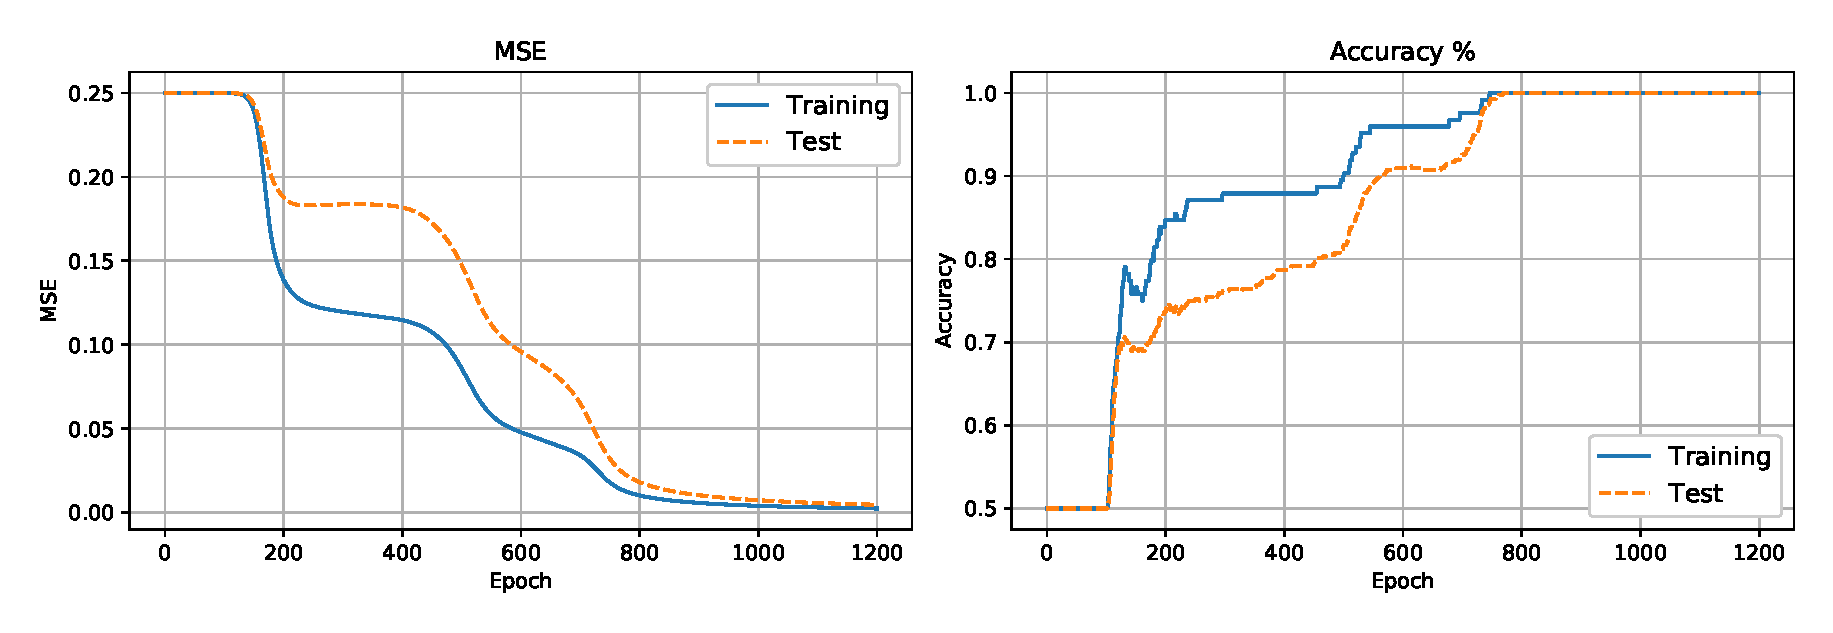
\includegraphics{Images/monks/monk1.eps}
                    }
                    \caption{MONK 1}
                    \label{fig:monk1}
                \end{subfigure}
                \begin{subfigure}{0.9\textwidth}
                    \resizebox{\textwidth}{!}{
                        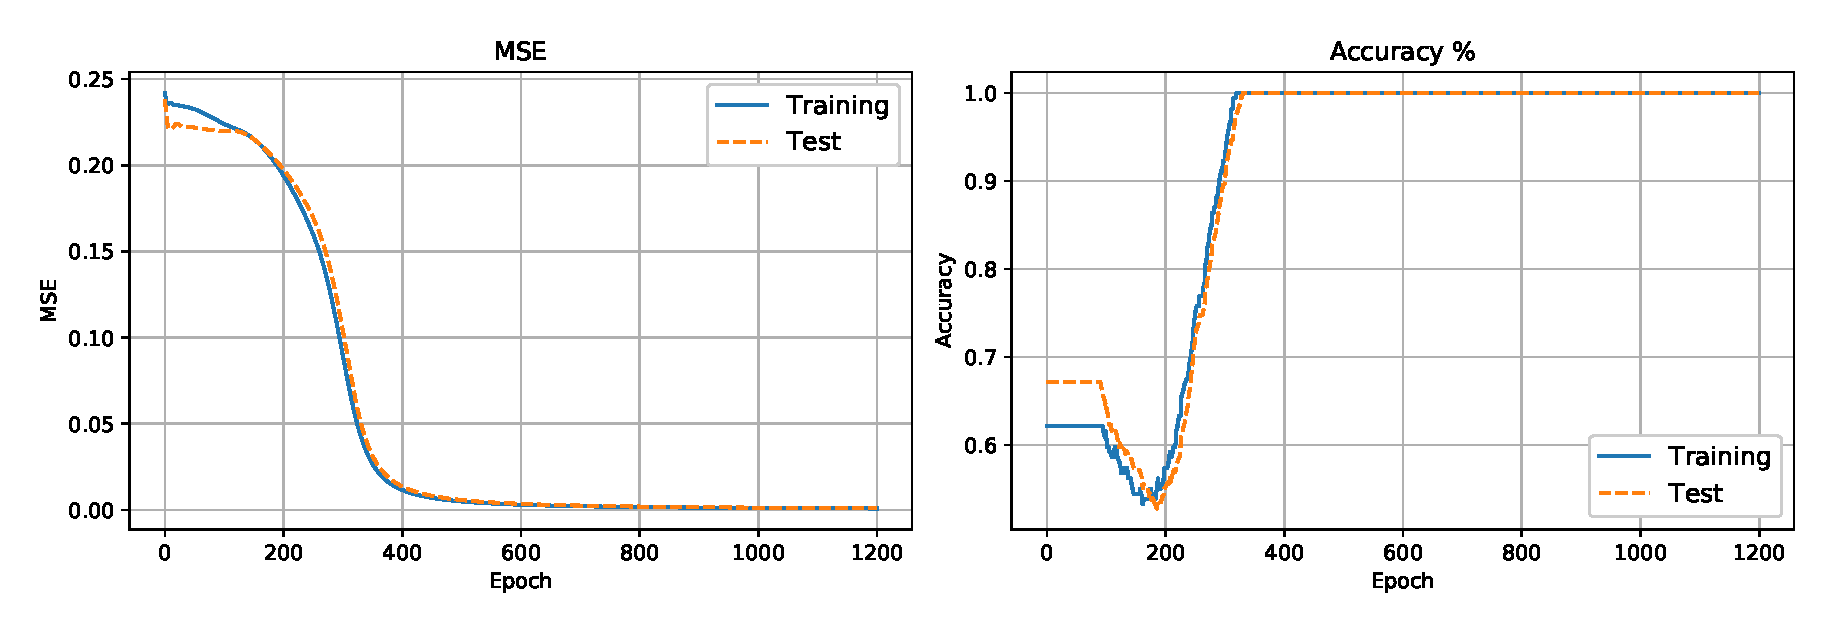
\includegraphics{Images/monks/monk2.eps}
                    }
                    \caption{MONK 2}
                    \label{fig:monk2}
                \end{subfigure}
                \begin{subfigure}{0.9\textwidth}
                    \resizebox{\textwidth}{!}{
   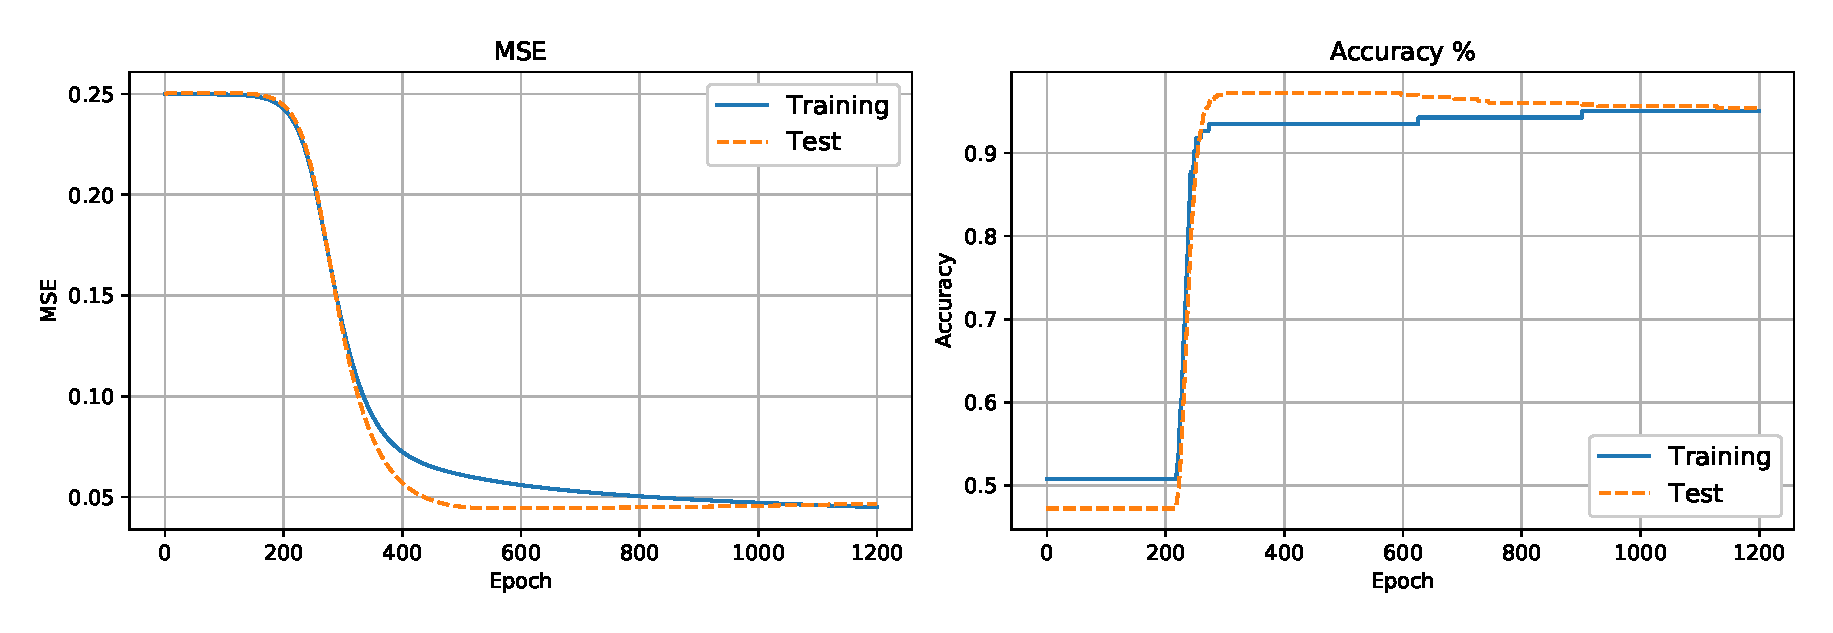
\includegraphics{Images/monks/monk3.eps}
                    }
                    \caption{MONK 3 without regularization}
                    \label{fig:monk3}
                \end{subfigure}
                \begin{subfigure}{0.9\textwidth}
                    \resizebox{\textwidth}{!}{
                        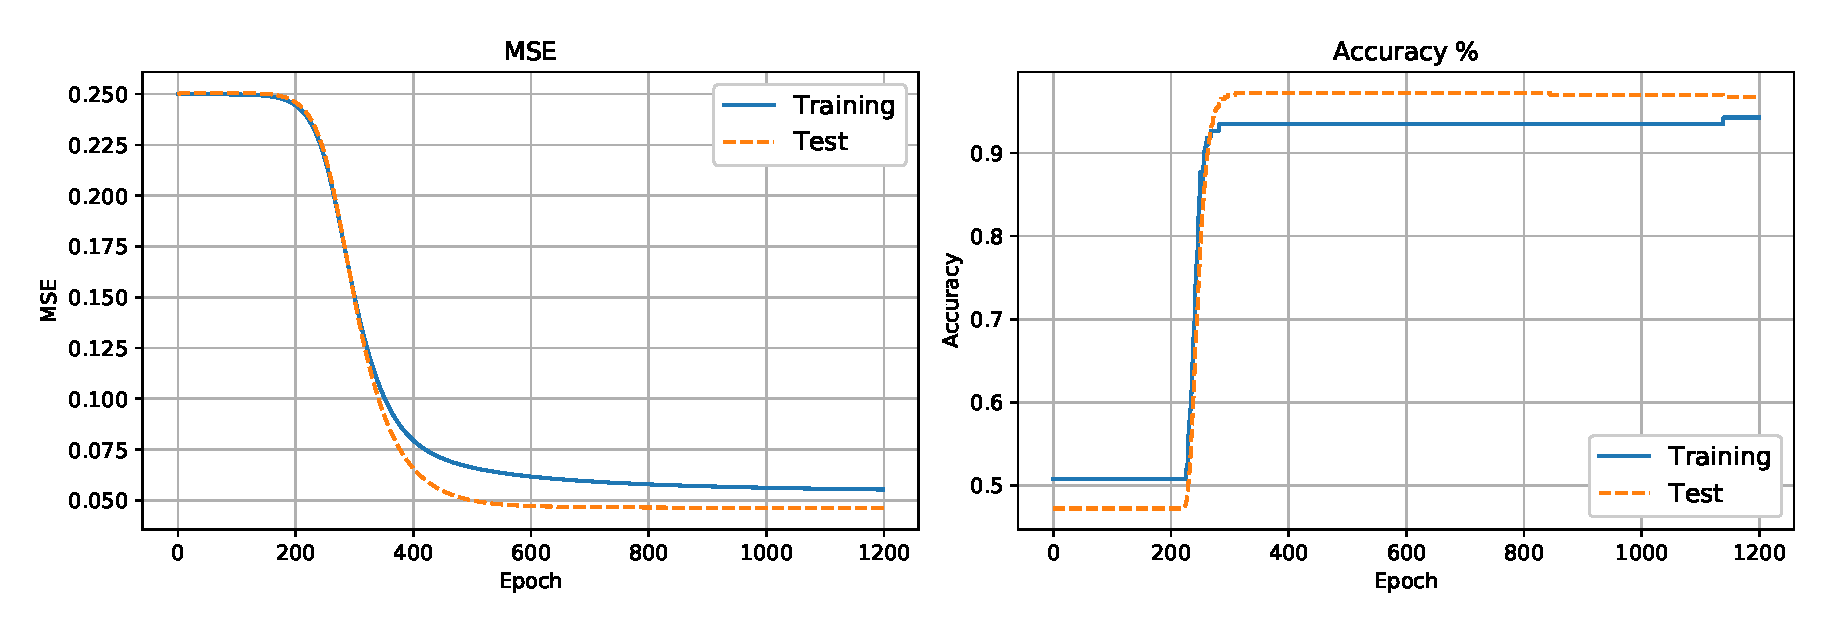
\includegraphics{Images/monks/monk3_reg.eps}
                    }
                    \caption{MONK 3 with regularization}
                    \label{fig:monk3_reg}
                \end{subfigure}
                
\caption{Plots of the MSE and Accuracy for the three MONK’s benchmarks.}
\label{fig:monk_plots} 
\end{figure}

\subsection{Cup Results}
\label{sec:cup}
For the experiments on the CUP dataset a shallow architecture was used: 10 (input units) - $\#units$ (hidden units) - 2 (output units). Where $\#units$ is a hyperparameter. We used the design set for all the stages that led to the model selection. Then, the internal test set was used for the model assessment.\\

\noindent\textbf{Screening Phase}:\\
To identify a good hyperparameters range a \emph{preliminary screening phase} has been performed by using the 15\% of the design set as the \emph{validation set}, and the remaining part as the \emph{training set}. During these trials, we manually changed the model’s hyperparameters and observed the resulting learning curves. We tried to achieve \emph{overfitting}, without using regularization approaches, and we noticed that, for a wide range of a different number of units, it is perfectly observable in 25000 epochs and so we decided to set the maximum number of epochs at 30000. Then, we saw the effects of the regularization on these overfitting models: with too small $\lambda$ values (e.g. 0.00001), the model still went into overfitting, while with too large $\lambda$ values (e.g. 0.0015), it risked going underfitting. We also noticed that, with too high $\eta$ values (e.g. 0.3), the models often overfit, and the curves have an initial instability (Fig.~\ref{fig:learning_rate_instability}). Finally, as regards the Nesterov momentum we have seen that, with the right $\alpha$ values, it can stabilize the curve (Fig.~\ref{fig:nm_fix_instability}) in the initial part (in the first 100 epochs) and accelerate convergence. On the other hand, with too large $\alpha$ and $\eta$ values, it can make the model overfits and shows instability. Moreover, we noticed that when the model goes overfitting, the validation curve, in the 30000 epochs, goes up without ever going down. Thus, as early stopping, we chose a small $\varepsilon_{GL}=0.009$ with $s_{UP}=200$. Some plots of underfitting and overfitting are shown in Fig.~\ref{fig:screening_cup}.

\begin{figure}[H]
    \centering
    \begin{subfigure}[b]{0.45\textwidth}
        \centering
        \resizebox{\textwidth}{!}{
               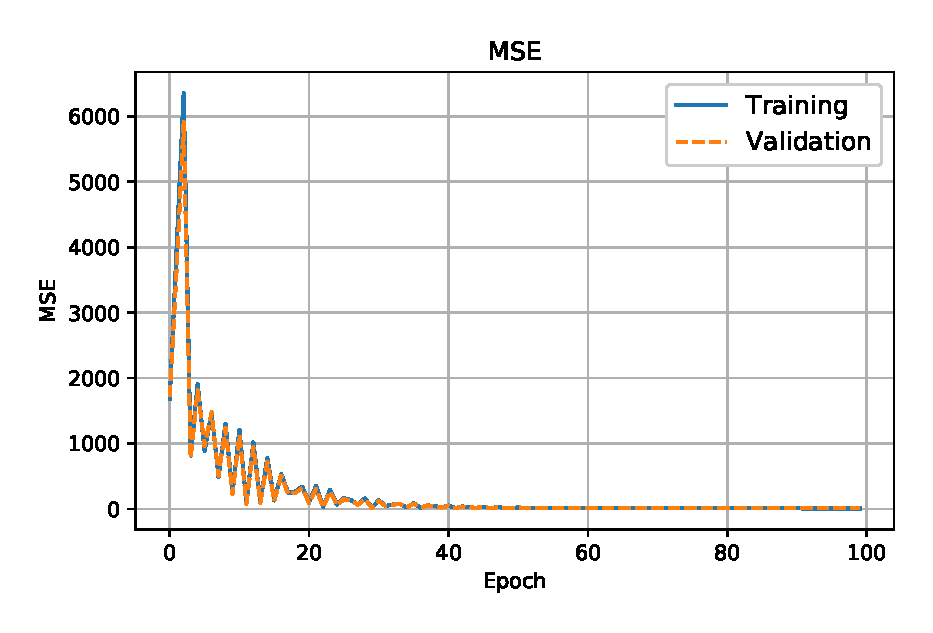
\includegraphics{Images/screening_phase/cup_instability_start.eps}
                    }
        \vspace{-0.74cm}
         \caption{From 0 to 100 epochs.}
         \label{fig:lr_inst_1}
    \end{subfigure}
    \hfill
    \begin{subfigure}[b]{0.45\textwidth}
        \centering
        \resizebox{\textwidth}{!}{
              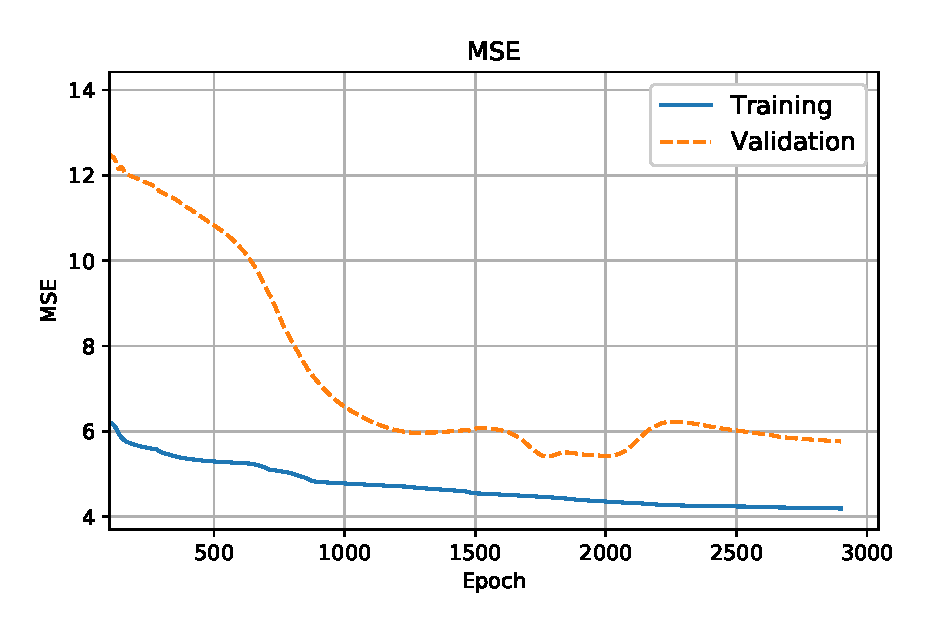
\includegraphics{Images/screening_phase/cup_instability_end.eps}
                    }
        \vspace{-0.74cm}
         \caption{From 100 to the end of training phase.}
         \label{fig:lr_inst_2}
     \end{subfigure}
        \vspace{-0.16cm}
\caption{Too high learning rate value can lead to instability in the training phase (e.g. 0.3 in this model).}
\label{fig:learning_rate_instability}
\end{figure}

\begin{figure}[H]
    \centering
    \begin{subfigure}[b]{0.45\textwidth}
        \centering
        \resizebox{\textwidth}{!}{
               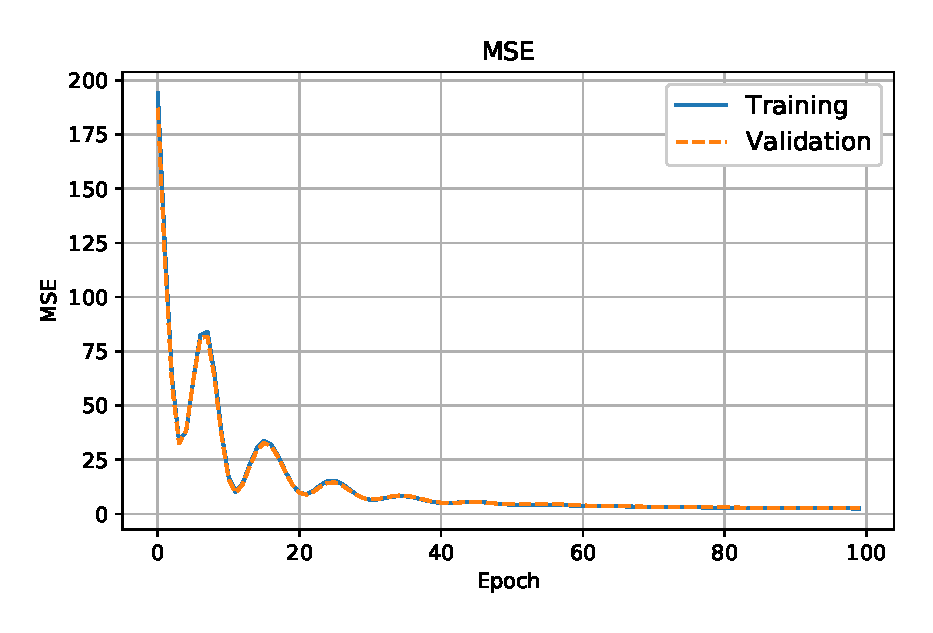
\includegraphics{Images/screening_phase/cup_no_momentum_start.eps}
                    }
        \vspace{-0.74cm}
         \caption{$\eta=0.01$ and No Momentum.}
         \label{fig:nm_fix_instability_1}
    \end{subfigure}
    \hfill
    \begin{subfigure}[b]{0.45\textwidth}
        \centering
        \resizebox{\textwidth}{!}{
              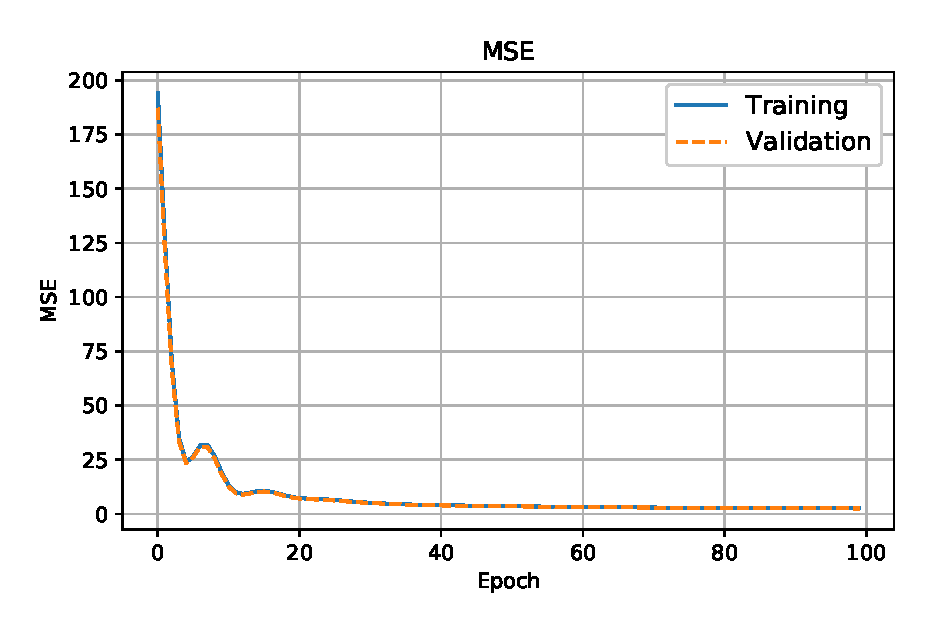
\includegraphics{Images/screening_phase/cup_with_nesterov_start.eps}
                    }
        \vspace{-0.74cm}
         \caption{$\eta=0.01$ and Nesterov Momentum with $\alpha=0.9$.}
         \label{fig:nm_fix_instability_2}
     \end{subfigure}
        \vspace{-0.16cm}
\caption{Nesterov momentum can make learning curves more stable. Model with \#units=50 and $\lambda=0$.}
\label{fig:nm_fix_instability}
\end{figure}


\begin{figure}[H]
    \centering
    \begin{subfigure}[b]{0.45\textwidth}
        \centering
        \resizebox{\textwidth}{!}{
               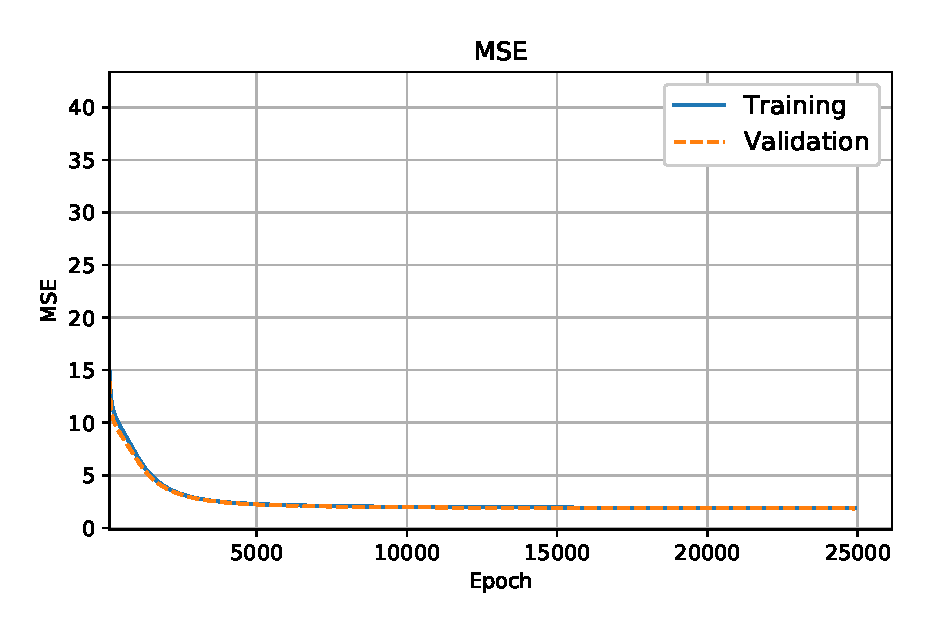
\includegraphics{Images/screening_phase/underfitting_10_1_end.eps}
                    }
        \vspace{-0.74cm}
         \caption{$\# units = 10,\,\, \eta = 0.002,\,\, \alpha = 0.1,\,\, \lambda = 0$}
         \label{fig:under_1}
    \end{subfigure}
    \hfill
    \begin{subfigure}[b]{0.45\textwidth}
        \centering
        \resizebox{\textwidth}{!}{
              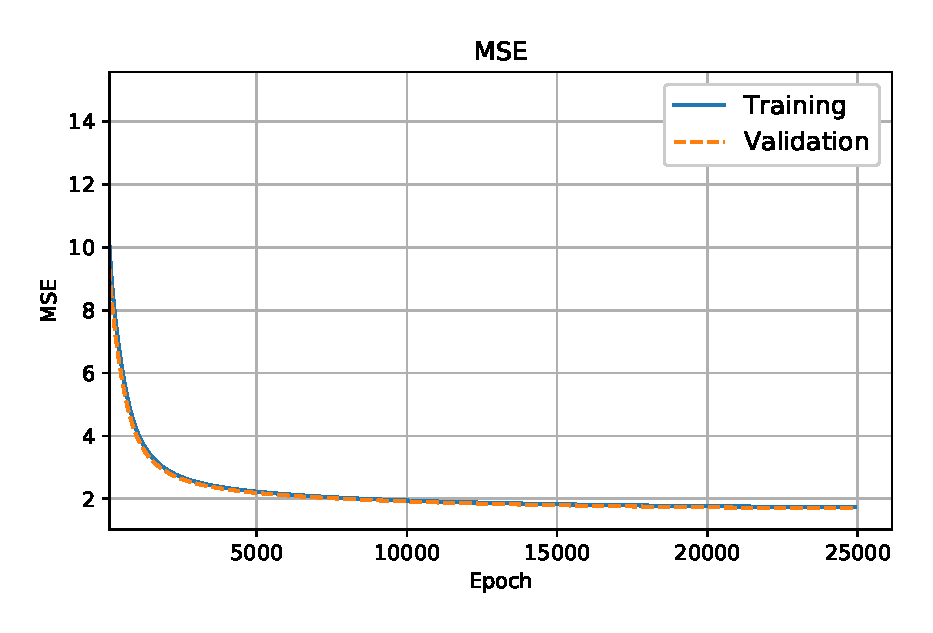
\includegraphics{Images/screening_phase/underfitting_20_1_end.eps}
                    }
        \vspace{-0.74cm}
         \caption{$\# units = 20,\,\, \eta = 0.002,\,\, \alpha = 0.3,\,\, \lambda = 0$}
         \label{fig:under_2}
     \end{subfigure}
     \begin{subfigure}[b]{0.45\textwidth}
         \centering
         \resizebox{\textwidth}{!}{
              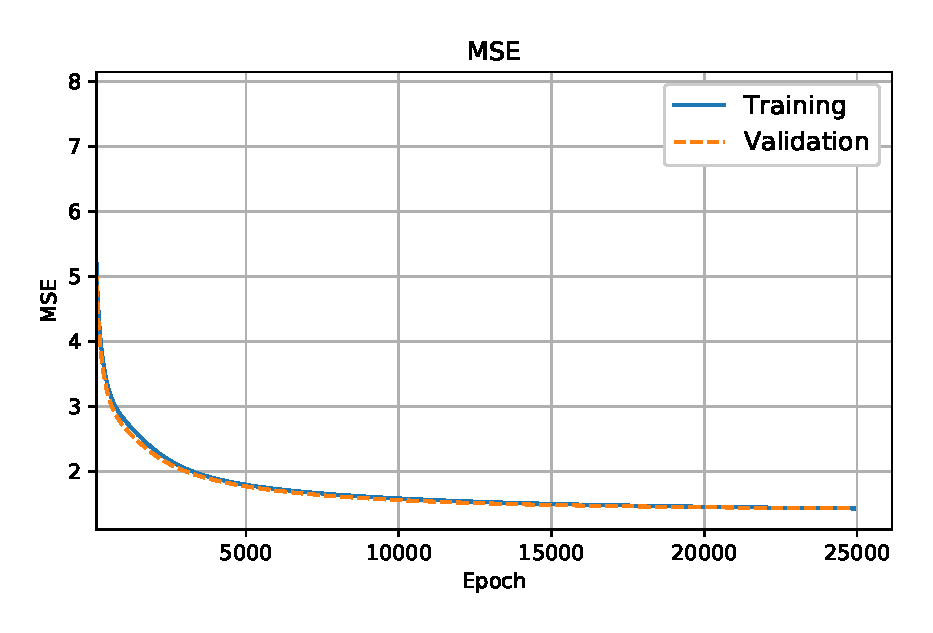
\includegraphics{Images/screening_phase/underfitting_50_1_end.eps}
                    }
        \vspace{-0.74cm}
         \caption{$\# units = 50,\,\, \eta = 0.007,\,\, \alpha = 0.2,\,\, \lambda = 0$}
         \label{fig:under_3}
     \end{subfigure}
     \hfill
     \begin{subfigure}[b]{0.45\textwidth}
         \centering
         \resizebox{\textwidth}{!}{                    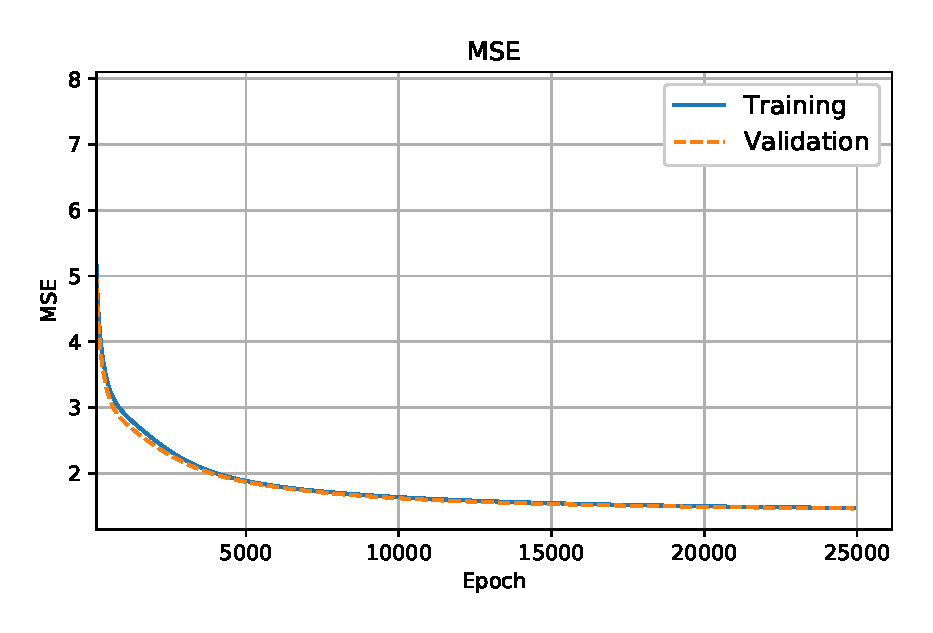
\includegraphics{Images/screening_phase/underfitting_80_1_end.eps}
                    }
        \vspace{-0.74cm}
         \caption{$\# units = 80,\,\, \eta = 0.005,\,\, \alpha = 0.4,\,\, \lambda = 0$}
         \label{fig:under_4}
     \end{subfigure}
        \vspace{-0.16cm}
    \begin{subfigure}[b]{0.45\textwidth}
        \centering
        \resizebox{\textwidth}{!}{
                        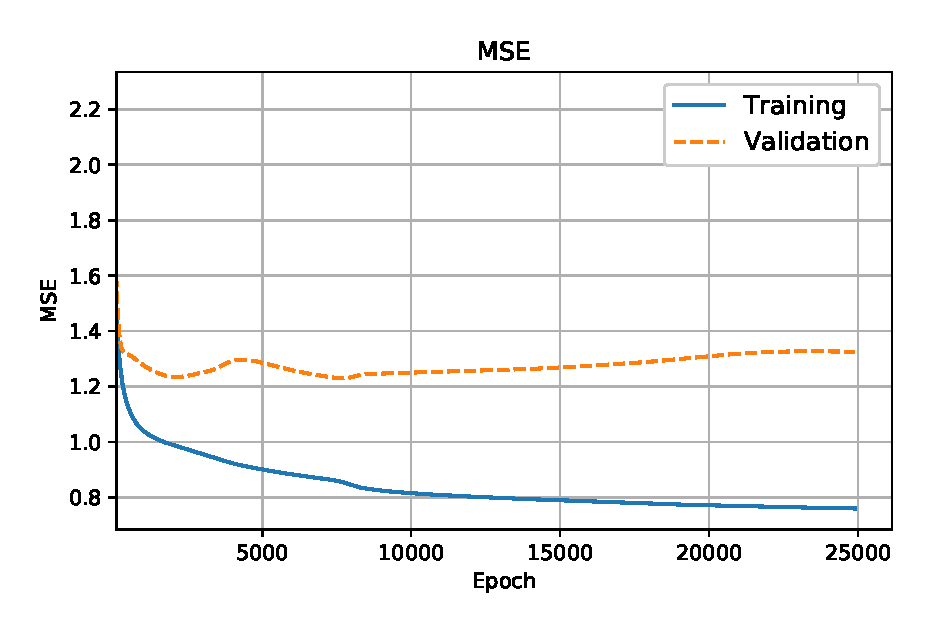
\includegraphics{Images/screening_phase/overfitting_100_1_end.eps}
                    }
         \caption{$\# units = 100,\,\, \eta = 0.07,\,\, \alpha = 0.8,\,\, \lambda = 0$}
         \label{fig:over_1}
    \end{subfigure}
    \hfill
    \begin{subfigure}[b]{0.45\textwidth}
        \centering
        \resizebox{\textwidth}{!}{
              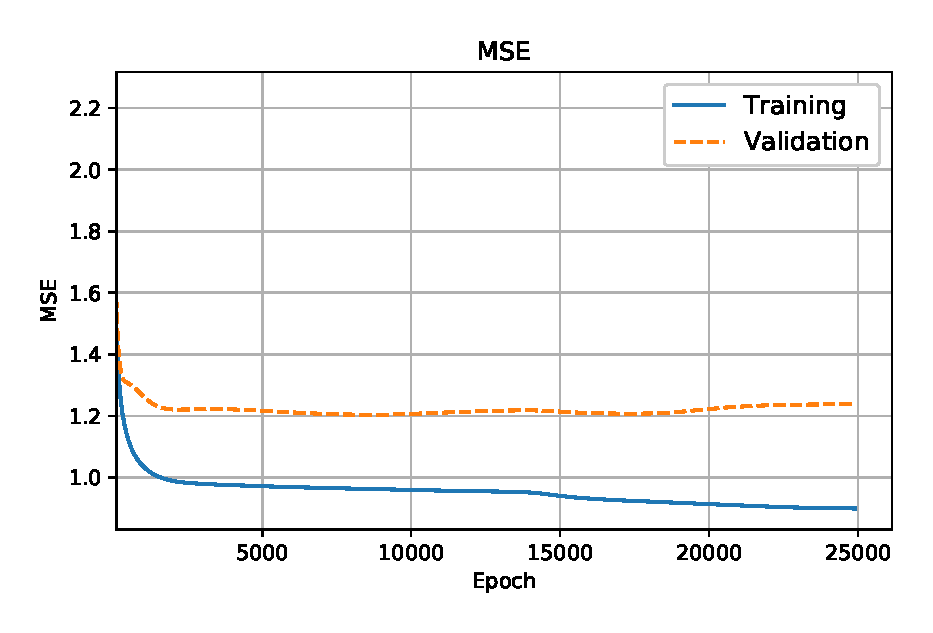
\includegraphics{Images/screening_phase/reg_100_1_end.eps}
                    }
         \caption{$\# units = 100,\, \eta = 0.07,\, \alpha = 0.8,\, \lambda = 0.0002$}
         \label{fig:reg_1}
     \end{subfigure}
     \begin{subfigure}[b]{0.45\textwidth}
         \centering
         \resizebox{\textwidth}{!}{
              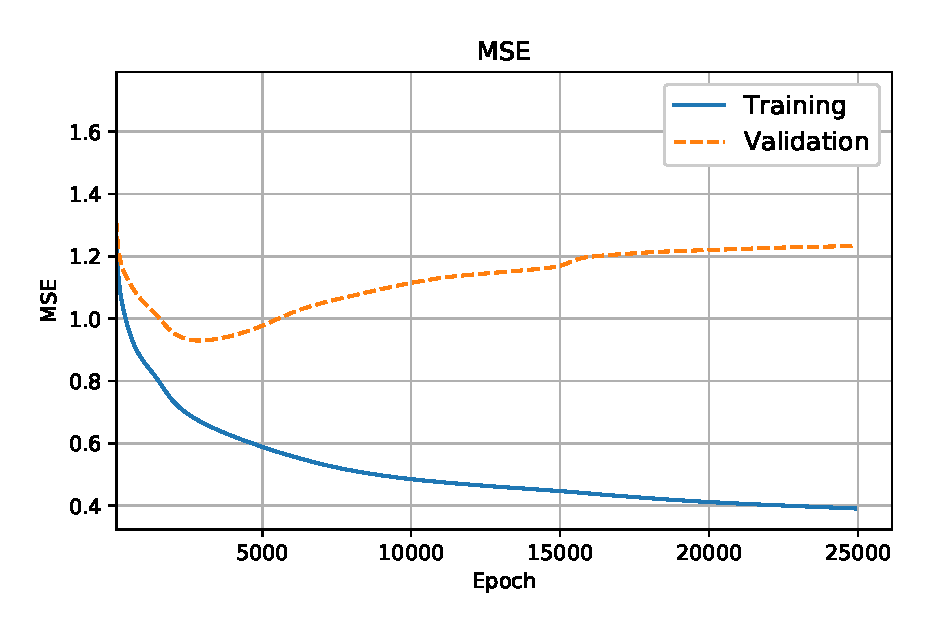
\includegraphics{Images/screening_phase/overfitting_50_1_end.eps}
                    }
         \caption{$\# units = 50,\,\, \eta = 0.06,\,\, \alpha = 0.9,\,\, \lambda = 0$}
         \label{fig:over_2}
     \end{subfigure}
     \hfill
     \begin{subfigure}[b]{0.45\textwidth}
         \centering
         \resizebox{\textwidth}{!}{                    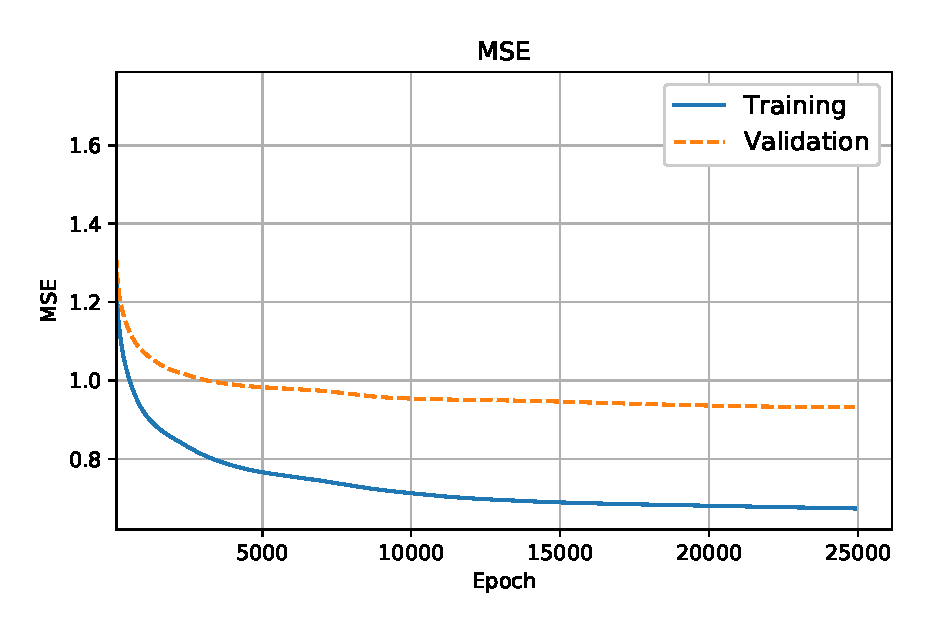
\includegraphics{Images/screening_phase/reg_50_1_end.eps}
                    }
         \caption{$\# units = 50,\,\, \eta = 0.06,\,\, \alpha = 0.9,\,\, \lambda = 0.0007$}
         \label{fig:reg_2}
     \end{subfigure}
     \centering
\begin{comment}
    \begin{subfigure}[b]{0.45\textwidth}
        \centering
        \resizebox{\textwidth}{!}{
                        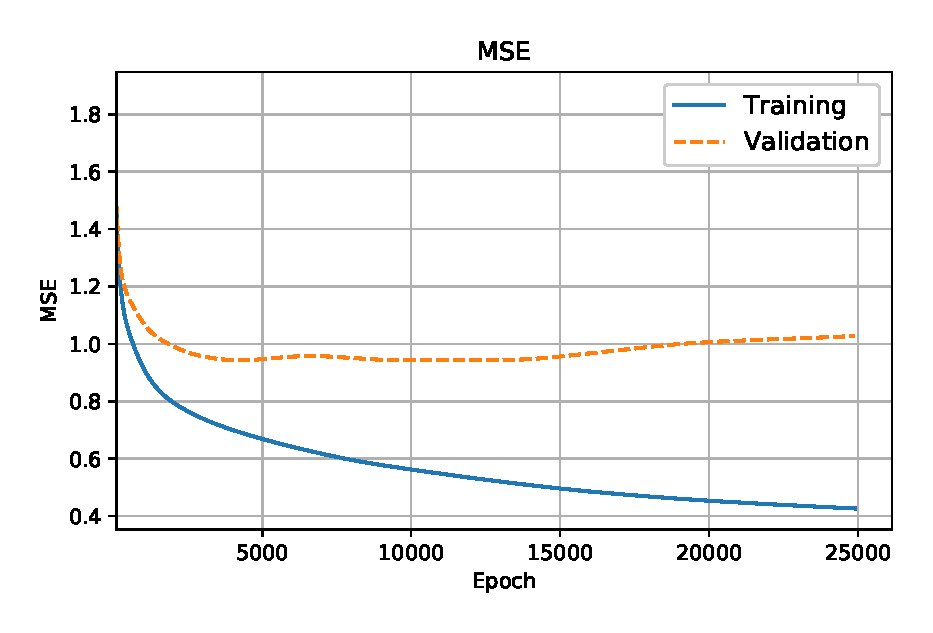
\includegraphics{Images/screening_phase/overfitting_50_2_end.eps}
                    }
         \caption{$\# units = 50,\,\, \eta = 0.04,\,\, \alpha = 0.9,\,\, \lambda = 0$}
         \label{fig:over_3}
    \end{subfigure}
    \hfill
    \begin{subfigure}[b]{0.45\textwidth}
        \centering
        \resizebox{\textwidth}{!}{
              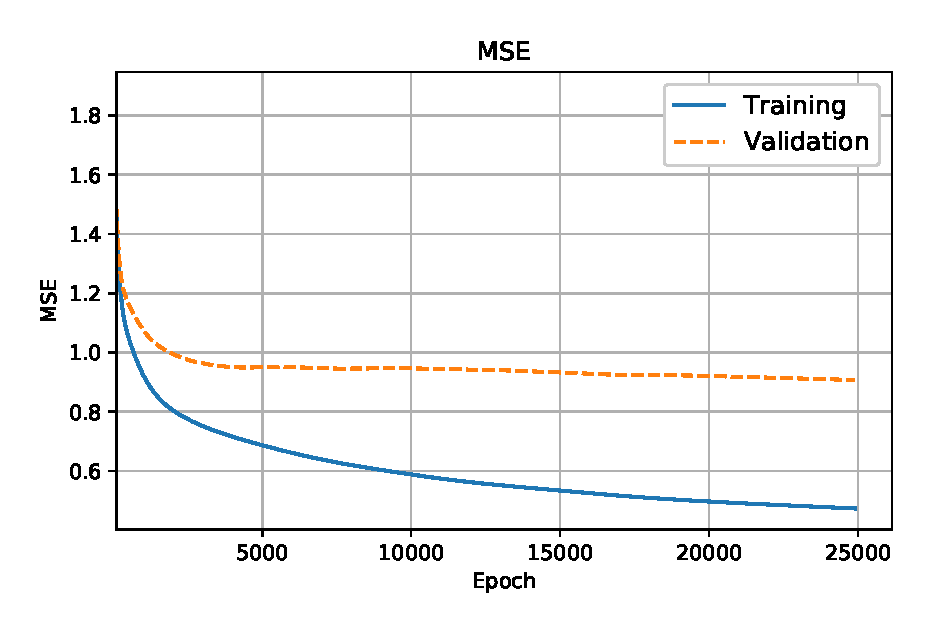
\includegraphics{Images/screening_phase/reg_50_2_end.eps}
                    }
         \caption{$\# units = 50,\,\, \eta = 0.04,\,\, \alpha = 0.9,\,\, \lambda = 0.00015$}
         \label{fig:oreg_3}
     \end{subfigure}
     \begin{subfigure}[b]{0.45\textwidth}
         \centering
         \resizebox{\textwidth}{!}{
              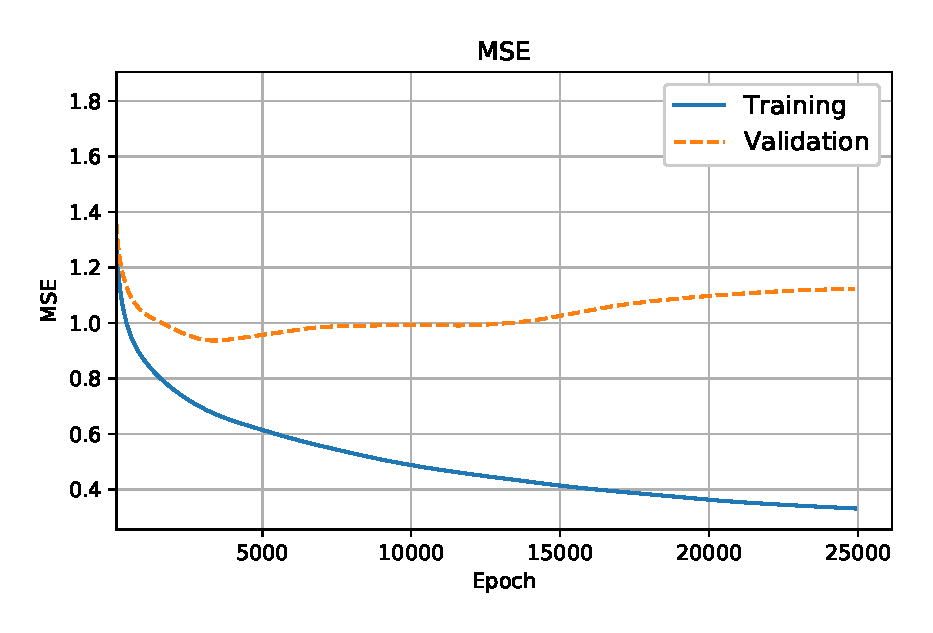
\includegraphics{Images/screening_phase/overfitting_80_1_end.eps}
                    }
         \caption{$\# units = 80,\,\, \eta = 0.05,\,\, \alpha = 0.9,\,\, \lambda = 0$}
         \label{fig:over_4}
     \end{subfigure}
     \hfill
     \begin{subfigure}[b]{0.45\textwidth}
         \centering
         \resizebox{\textwidth}{!}{                    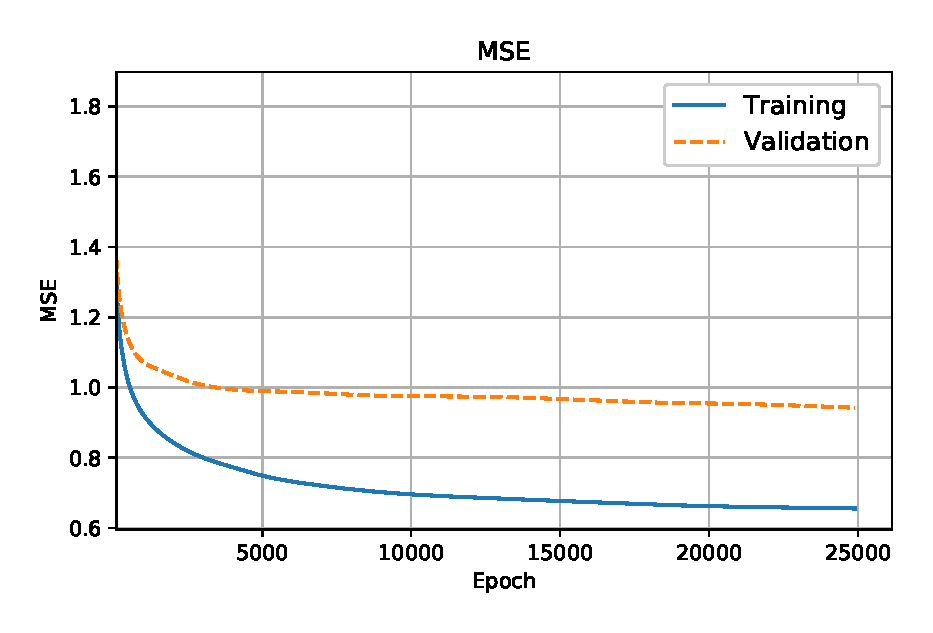
\includegraphics{Images/screening_phase/reg_80_1_end.eps}
                    }
         \caption{$\# units = 80,\,\, \eta = 0.05,\,\, \alpha = 0.9,\,\, \lambda = 0.0005$}
         \label{fig:reg_4}
     \end{subfigure}
\end{comment}
     \caption{Examples of underfitting (\ref{fig:under_1}, \ref{fig:under_2}, \ref{fig:under_3}, \ref{fig:under_4}), overfitting (\ref{fig:over_1}, \ref{fig:over_2}) models and their regularized versions (\ref{fig:reg_1}, \ref{fig:reg_2}). Plots have been generated from the 100th epochs to better visualize the behaviour of the learning curves.}
     \label{fig:screening_cup}
\end{figure}

\noindent\textbf{Large Grid Search}:\\
From the screening phase we were able to isolate some ranges and run a grid search with the hyperparameters reported in Tab.~\ref{tab:large_grid} using a 4-fold CV. Tab.~\ref{tab:large_grid_result} shows the six best hyperparameter combinations found using the estimate of the MEE on the validation set as a goodness criterion. We can see that the best performances were obtained with a number of units from 40 to 100, learning rate from 0.03 to 0.06, momentum from 0.6 to 0.9 and regularization from 0.0001 to 0.0005. Based on these results, we can shrink the hyperparameters ranges and perform a finer grid search with the same criteria and the ranges reported in Tab.~\ref{tab:finer_grid}.

\begin{table}[H]
\small
    \centering
    \begin{tabular}{ |c|c| }
        \hline
        \textbf{Hyperparameters} & \textbf{Values range}\\
        \hline
        \hline
        \textbf{\# units} & 20, 40, 80, 100, 150\\
        \hline
         $\boldsymbol{\eta}$ & 0.03, 0.06, 0.08, 0.098\\
        \hline
        $\boldsymbol{\alpha}$ & 0.2, 0.4, 0.6, 0.8, 0.9\\
        \hline
        $\boldsymbol{\lambda}$ & 0.0001, 0.0005, 0.0009, 0.0013\\
        \hline
        \textbf{Epochs} & 30000\\
        \hline
        \textbf{Early Stop} & ($\varepsilon_{GL}$ = 0.009, $s_{UP}$ = 200)\\
        \hline
    \end{tabular}
    \caption{Range of Hyper-parameters for the large grid search}
    \label{tab:large_grid}
\end{table}

\begin{table}[H]
\small
    \centering
    \begin{tabular}{ |c|c|c|c|c|c|c|c|c|  }
     \hline
     \multicolumn{9}{|c|}{\textbf{Scoring Large Grid Search with 4 Folds }} \\
     \hline
      \hline
       \textbf{} & \textbf{\# units} & $\boldsymbol{\eta}$ & $\boldsymbol{\alpha}$ & $\boldsymbol{\lambda}$& \textbf{MEE (TR)} & \textbf{MEE (VL)} & \textbf{MEE (Int. TS)} & \textbf{TR Time (s)}\\
     \hline
    cup L1 & 80 & 0.06  & 0.6 & 0.0001 & $0.878 \pm 0.040$ & $1.076 \pm 0.035$ & $1.031 \pm 0.015$ & $186.4 \pm 65.7$ \\
    \hline
    cup L2 & 40 & 0.06  & 0.9 & 0.0005 & $0.879 \pm 0.046$ & $1.084 \pm 0.045$ & $1.016 \pm 0.012$ & $52.9 \pm 30.1$\\
    \hline
    cup L3 & 80 & 0.03  & 0.8 & 0.0001 & $0.903 \pm 0.048$ & $1.090 \pm 0.023$ & $1.041 \pm 0.015$ & $160.4 \pm 71.2$\\
    \hline
    cup L4 & 40 & 0.03  & 0.9 & 0.0001 & $0.887 \pm 0.043$ & $1.094 \pm 0.027$ & $1.050 \pm 0.021$ & $24.9 \pm 8.1$\\
    \hline
    cup L5 & 80 & 0.03  & 0.9 & 0.0001 & $0.870 \pm 0.042$ & $1.094 \pm 0.032$ & $1.042 \pm 0.033$ & $49.5 \pm 14.7$\\
    \hline
    cup L6 & 100 & 0.03 & 0.9 & 0.0001 & $0.859 \pm 0.107$ & $1.095 \pm 0.016$ & $1.061 \pm 0.019$ & $94.7 \pm 77.2$\\
     \hline
    \end{tabular}
    \caption{Best six hyperparameter combination obtained from the large grid search.}
    \label{tab:large_grid_result}
\end{table}

\noindent\textbf{Finer Grid Search}:\\
Tab.~\ref{tab:finer_grid_results} shows the top three best hyperparameter combinations found in the finer grid search.

\begin{table}[H]
\small
    \centering
    \begin{tabular}{ |c|c| }
        \hline
        \textbf{Hyperparameters} & \textbf{Values range}\\
        \hline
        \hline
        \textbf{\# units} & 40, 50, 60, 70, 80, 90, 100\\
        \hline
         $\boldsymbol{\eta}$ & 0.03, 0.034, 0.038, 0.042, 0.046, 0.050, 0.054, 0.058, 0.06\\
        \hline
        $\boldsymbol{\alpha}$ & 0.6, 0.7, 0.8, 0.99\\
        \hline
        $\boldsymbol{\lambda}$ & 0.0001, 0.0002, 0.0003, 0.0004, 0.0005\\
        \hline
        \textbf{Epochs} & 30000\\
        \hline
        \textbf{Early Stop} & ($\varepsilon_{GL} = 0.009$, $s_{UP} = 200$)\\
        \hline
    \end{tabular}
    \caption{Hyperparameters ranges for the finer grid search.}
    \label{tab:finer_grid}
\end{table}

\begin{table}[H]
\small
    \centering
    \begin{tabular}{ |c|c|c|c|c|c|c|c|c|  }
     \hline
     \multicolumn{9}{|c|}{\textbf{Scoring Finer Grid Search on 4 Folds}} \\
     \hline
     \hline
      \textbf{} & \textbf{\# units} & $\boldsymbol{\eta}$ & $\boldsymbol{\alpha}$ & $\boldsymbol{\lambda}$& \textbf{MEE (TR)} & \textbf{MEE (VL)} & \textbf{MEE (Int. TS)} & \textbf{TR Time (s)}\\
     \hline
      cup F1 & 50 & 0.058  & 0.9 & 0.0005 & $0.865 \pm 0.048$ & $1.061 \pm 0.015$ & $1.013 \pm 0.020$ & $49.10 \pm 21.07$  \\
      \hline
      cup F2 & 50 & 0.058  & 0.9 & 0.0004 & $0.867 \pm 0.045$ & $1.065 \pm 0.028$ & $1.028 \pm 0.016$ & $31.52 \pm 13.76$ \\
      \hline
      cup F3 & 70 & 0.054  & 0.9 & 0.0004 & $0.905 \pm 0.070$ & $1.068 \pm 0.042$ & $1.018 \pm 0.015$ & $78.88 \pm 91.18$ \\
      \hline
    \end{tabular}
    \caption{Best three hyperparameter combination obtained from the finer grid search.}
    \label{tab:finer_grid_results}
\end{table}

\noindent\textbf{Final model selection}:\\
We choose the hyperparameter combination of \emph{cup F1} as hyperparameters of the final model because, in Tab.~\ref{tab:finer_grid_results}, it is the one with the lowest estimate of the MEE on the validation set.
So, we re-trained \emph{cup F1} on 90\% of the design set, leaving the remaining 10\% as a validation set for early stopping techniques. We repeated the re-training for ten trials to avoid bad weights initialization and we selected the model with the minimum MEE validation error. Tab.~\ref{tab:final_model} shows the MEE values of the retraining (training and validation), the result of the \textit{Model Assessment} performed on the \textit{internal test set}, and the computing time during the final re-training.  Also, the learning curves for training and validation have been included in Fig.~\ref{fig:final_model_plot}, where we can observe smooth behaviour during training.
\begin{table}[H]
\small
    \centering
    \begin{tabular}{ |c|c|c|c|c|c|c|c|  }
     \hline
     \textbf{\# units} & $\boldsymbol{\eta}$ & $\boldsymbol{\alpha}$ & $\boldsymbol{\lambda}$& \textbf{MEE (TR)} & \textbf{MEE (VL)} & \textbf{MEE (Internal TS)}& \textbf{TR Time (s)}\\
     \hline
      50 & 0.058  & 0.9 & 0.0005 & $0.85648$ & $0.960216$ & $0.99397$ & 54 \\
      \hline
    \end{tabular}
    \caption{Results of the final model retrained on the 90\% design set and the Model Assessment on the internal test set.}
    \label{tab:final_model}
\end{table}

\begin{figure}[H]
    \centering
    \begin{subfigure}[b]{0.45\textwidth}
        \centering
        \resizebox{\textwidth}{!}{
              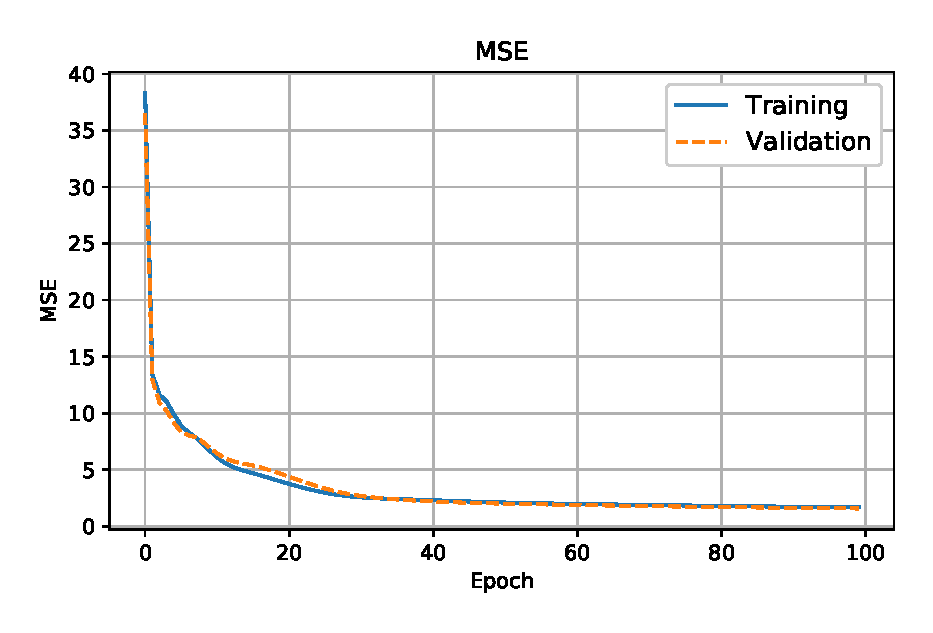
\includegraphics{Images/final_model/model_7_start.eps}
                    }
         \caption{From 0 to 100 epochs.}
         \label{fig:final_model_plot_0_100}
    \end{subfigure}
    \hfill
    \begin{subfigure}[b]{0.45\textwidth}
        \centering
        \resizebox{\textwidth}{!}{
               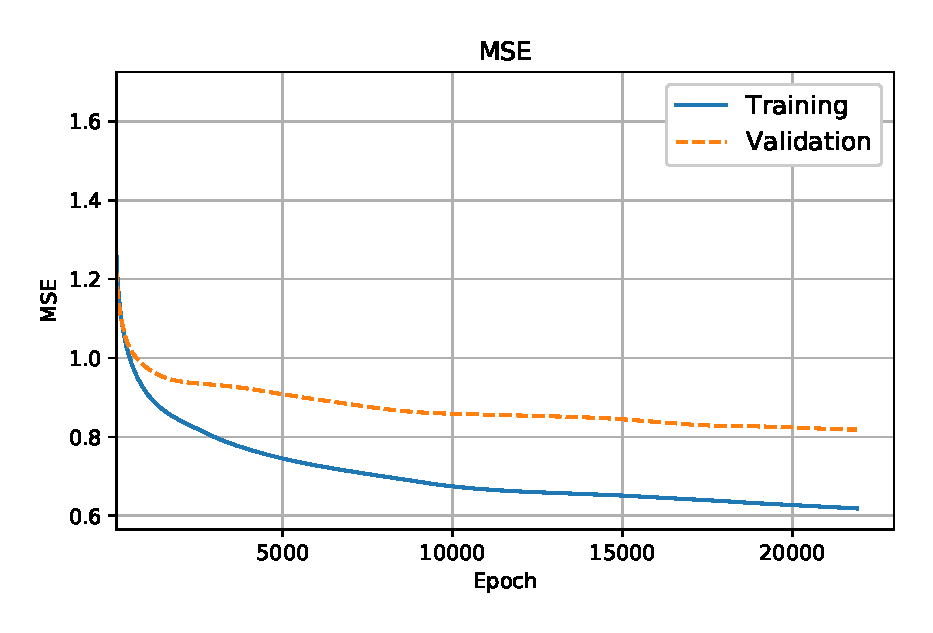
\includegraphics{Images/final_model/model_7_end.eps}
               }
         \caption{From 100 to 22005 epochs.}
         \label{fig:final_model_plot_100_to_end}
     \end{subfigure}
     \begin{subfigure}[b]{0.45\textwidth}
         \centering
         \resizebox{\textwidth}{!}{
              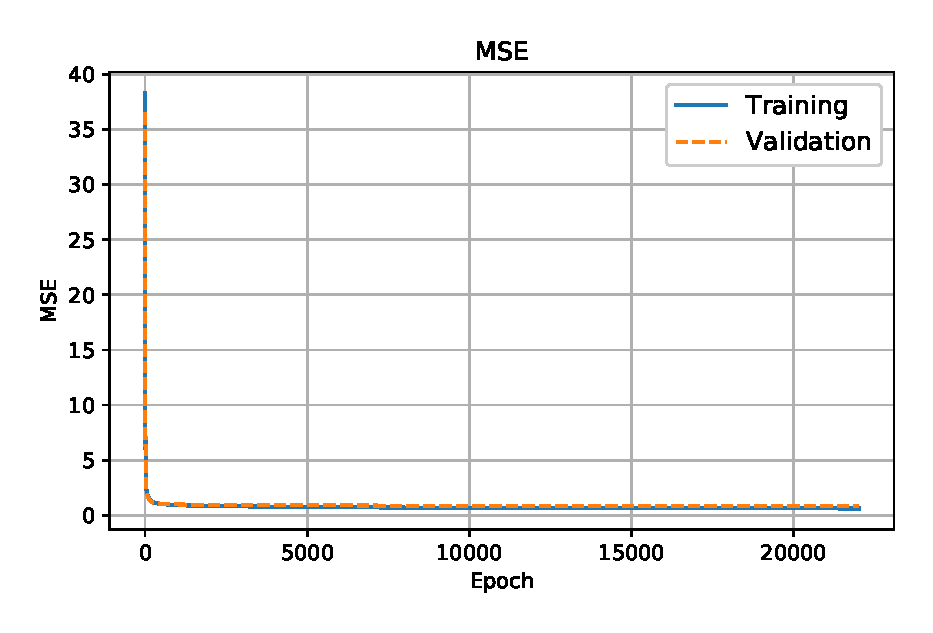
\includegraphics{Images/final_model/model_7_all.eps}
                    }
         \caption{Full plot with all the epochs.}
         \label{fig:final_model_plot_all}
     \end{subfigure}
\caption{Final model plots. To better observe the learning curves behaviors, in addition to the complete plot (\ref{fig:final_model_plot_all}), the plots from 0 to 100 epochs (\ref{fig:final_model_plot_0_100}) and 100 to 22005 epochs (\ref{fig:final_model_plot_100_to_end}) (when the training phase ends) have been added.}
     \label{fig:final_model_plot}
\end{figure}
Finally, to generate the prediction on the "blind test set", we re-trained the model on the initial training dataset (design set plus internal test set), excluding 10\% of the data as validation for the same reason as above. The results are in \texttt{isanet\_ML-CUP19-TS.csv}.


\begin{comment}
\noindent\textbf{Explorer grid}\\
we fixed some range and we did cross validation on it, just to observe how the error change with different combination of paramenter. After that we extrated the range of min and max value for each hyperparamter with a error = 1.0. We observed how the learning rate changed with the momentum: indirect proportion. So we extrated the min and max value for the lr for each momentum. With this interval we decided to run a kfold cross validation in order to see....\\

\noindent\textbf{init grid}
\begin{itemize}
    \item we observed that 13000 epoch are enough for every kind of expirement, to reach overfitting, underfittig, ecc...
    \item we tried different parameters to see which one allow to reach overfitting and underfittin in order to find some interval for a init grid search
    \item we observed that with a learning rate $\ge 0.1$ models with different number of units are very unstable, is easy to reach overfitting and underfitting under 1000 epoch with high mse.
    \item so as upper bound for a init grid search we seetted as learning rate: $0.99$
    \item we observed that with  $0.002\leq lr \leq 0.007$ with different number of units the convergence is very slow, we need more then 13000 epoch and we never reach overfitting, error is high (1.3/1.4) 
    \item the goal in this phase is not to find the minimium of the generalizzation but to find better intervals for a final grid search. we want to see if there is some parameters that give us low error.
    
\end{itemize}

\textbf{final grid}\\
\end{comment}


\section{Conclusions}
\label{sec:conclusions}
During the development of the IsaNet, we have become increasingly familiar with the theory learned in class. In particular, we enjoyed the screening phase, because let us better understand the real influence that the hyperparameters have in the training phase. For example, we fully grasped the power of Tikhonov regularization after implementing and testing it in various cases. We mainly focused on writing a reliable library, so that we can use it in future works as well, and we preferred to work with quite standard neural networks for our first approach to Machine Learning. Despite this, we were pleased to insert something extra in the appendices.

As regards future work: it would be interesting to see how the result on the CUP varies using Super Accelerated Nesterov, or trying neural networks with more than one hidden layer. We would also have liked to try the Conjugate Gradient and the Quasi-Newton, but for lack of time, we had to give it up.

\section*{Acknowledgments}
We agree to the disclosure and publication of my name, and of the results with preliminary and final ranking. 
\bibliography{references} 

\newpage
\begin{appendices}
\section{Comparisons between Momentum Methods}
\label{appendix:momentum_comp}
The delta rule, at iteration $i+1$, using the gradient descent algorithm with the Classic  heavy-ball Momentum \cite{Polyak1964}, Nesterov \cite{sutskever2013} and Accelerated Nesterov Momentum \cite{nakerst2020gradient} can be summarized in this way:
$$ \Delta^i = \alpha\Delta^{i-1} - \eta\nabla L(w^i +\sigma\Delta^{i-1})$$
$$ w^{i+1} = w^i + \Delta^i$$

When $\sigma = 0$, the delta rule uses the heavy-ball method, and when $\sigma = \alpha$, the Nesterov momentum is used. In \cite{nakerst2020gradient} is shown that can be advantageous to use values of $\sigma$ larger than $\alpha \approx 1$. Instead of using the gradient at an estimated point one step ahead, the gradient is computed at a much further estimated point. This corresponds to an extension of Nesterov and that is why it is called \emph{Accelerated Nesterov Momentum}. Figure \ref{fig:monk1_4_momentum} shows the effect of momentum methods.
\begin{figure}[H]
    \centering
    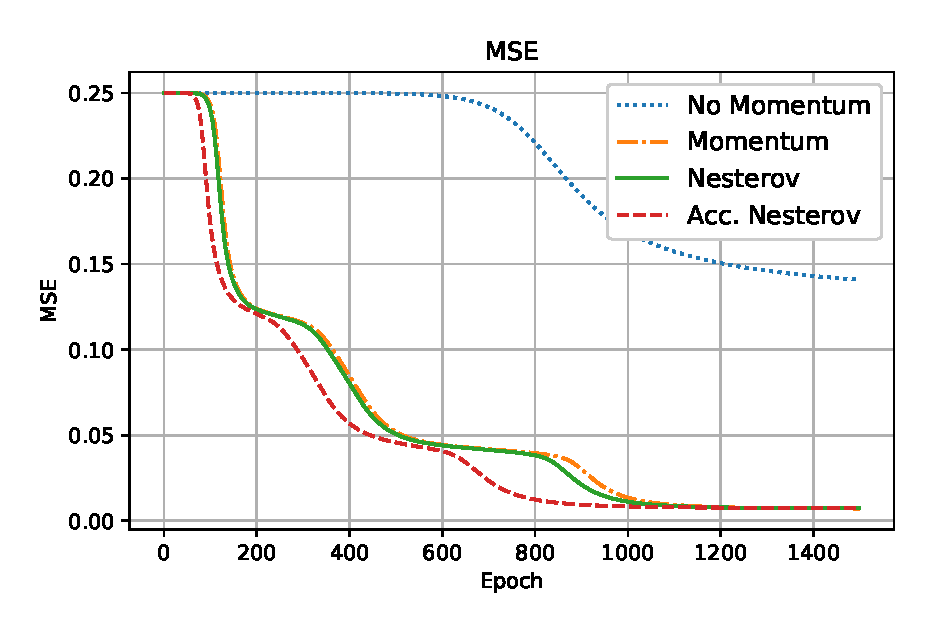
\includegraphics[scale = 0.8]{Images/monk1_4_momentum.eps}
    \caption{Training Learning curves using Monk 1 as dataset with different momentum methods. To compare the learning curves and correctly observe the convergence speed, all the models have been trained starting from the same initial weights.}
    \label{fig:monk1_4_momentum}
\end{figure}
\newpage

\section{Code Examples}
\label{appendix:code_example}
\begin{listing}[!ht]
\inputminted{python}{code/low_api.py}
\caption{A low level API example on the Monk 1 dataset.}
\label{listing:low_api}
\end{listing}

\begin{listing}[!ht]
\inputminted{python}{code/high_api.py}
\caption{A high level API example on the Monk 1 dataset.}
\label{listing:high_api}
\end{listing}

\begin{listing}[!h]
\inputminted{python}{code/model_selection.py}
\caption{Model Selection API example on the CUP dataset.}
\label{listing:model_selection}
\end{listing}

\section{MONKS}
\label{appendix:monks}
\begin{figure}[H]
    \centering
                \begin{subfigure}{0.9\textwidth}
                    \resizebox{\textwidth}{!}{
                        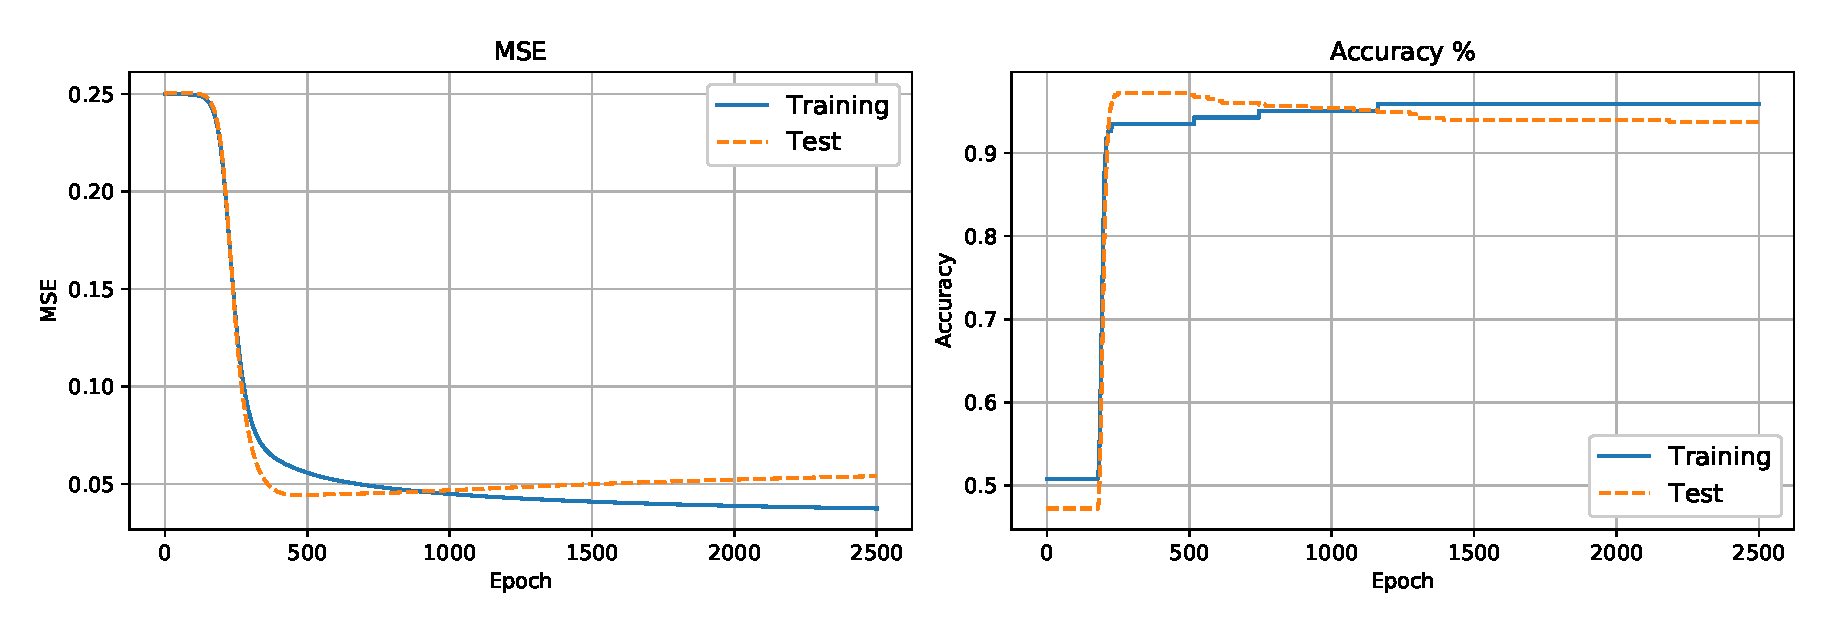
\includegraphics{Images/monks/monk3_overfitting.eps}
                    }
                    \caption{MONK 3 with no regularization}
                    \label{fig:monk3_app}
                \end{subfigure}
                \begin{subfigure}{0.9\textwidth}
                    \resizebox{\textwidth}{!}{
                        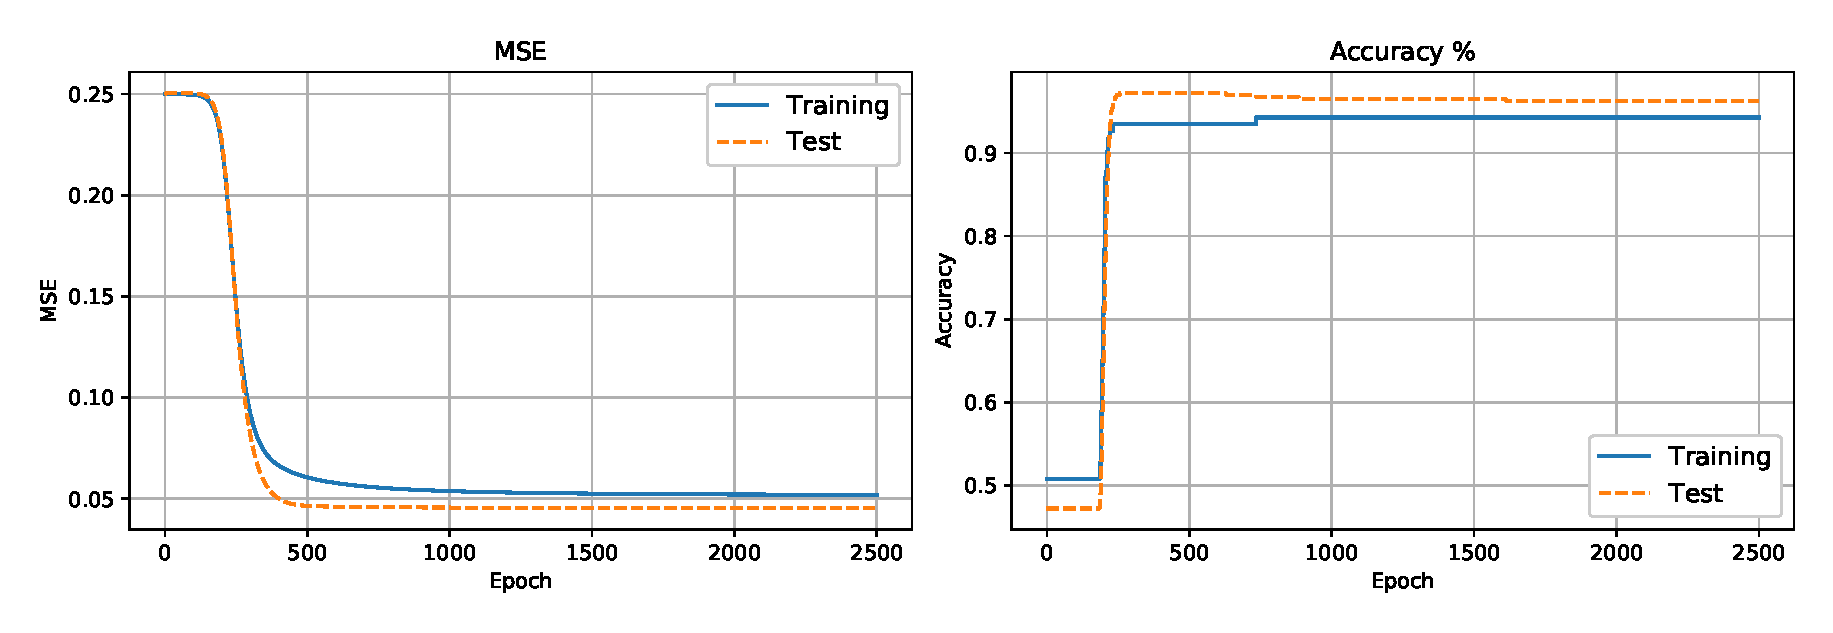
\includegraphics{Images/monks/monk3_over_reg.eps}
                    }
                    \caption{MONK 3 with regularization}
                    \label{fig:monk3_reg_app}
                \end{subfigure}
\caption{Plot of the MSE and accuracy for the MONK 3. In Fig.~\ref{fig:monk3_app}, the model without regularization goes into \emph{overfitting} just before 1000 epochs. Indeed the generalization error measured over the test examples increases, even as the error over the training examples continues to decrease. In Fig.~\ref{fig:monk3_reg_app} is shown how the regularization prevents overfitting.}
\label{fig:monk3_appendix} 
\end{figure}

\begin{table}[h]
\small
    \centering
    \begin{tabular}{ |c|c|c|c|c|c|c|c|c|  }
      \hline
       \textbf{Task} &\textbf{Topology}&\textbf{Batch size}& $\boldsymbol{\eta}$ & $\boldsymbol{\alpha}$ & $\boldsymbol{\lambda}$& \textbf{MSE(TR/TS)} & \textbf{Accuracy(TR/TS)($\boldsymbol{\%}$)}\\
     \hline
    MONK 1 &17$\rightarrow$4$\rightarrow$1 & 1 & 0.4 & 0.8  & 0 & 0.00016 / 0.00023 & 100\% / 100\%\\
    \hline
    MONK 1 &17$\rightarrow$10$\rightarrow$1 & 1 & 0.4 & 0.7  & 0 & 0.00012 / 0.00017 & 100\% / 100\%\\
    \hline
    MONK 1 & 17$\rightarrow$4$\rightarrow$1 & 31 & 0.6 & 0.7  & 0 & 0.00115 / 0.00182 & 100\% / 100\%\\
    \hline
    MONK 2 & 17$\rightarrow$3$\rightarrow$1& 1 & 0.1 & 0.4  & 0 & 0.00205 / 0.00235 & 100\% / 100\%\\
    \hline
    MONK 2 & 17$\rightarrow$10$\rightarrow$1& 1 & 0.1 & 0.4  & 0 & 0.00197 / 0.00229 & 100\% / 100\%\\
    \hline
    MONK 2 & 17$\rightarrow$3$\rightarrow$1& 68 & 0.1 & 0.4  & 0 & 0.00301 / 0.00349 & 100\% / 100\%\\
    \hline
    MONK 2 & 17$\rightarrow$3$\rightarrow$1& 169 & 0.01 & 0.9  & 0 & 0.00970 / 0.01217 & 100\% / 100\%\\
    \hline
    MONK 3 (no reg.)&17$\rightarrow$4$\rightarrow$1 &1 & 0.01 & 0.6  & 0 & 0.04519 / 0.04536 & 95\% / 95\%\\
    \hline
    MONK 3 (no reg.)&17$\rightarrow$10$\rightarrow$1 &1 & 0.01 & 0.5  & 0 & 0.04828 / 0.04398 & 95\% / 95\%\\
    \hline
    MONK 3 (no reg.) & 17$\rightarrow$4$\rightarrow$1&61 &0.6 & 0.3 & 0 & 0.04904 / 0.04483 & 94\% / 96\%\\

     \hline
    \end{tabular}
    \caption{Preliminary cases discovered during the screening phase of the MONKS dataset. Normal momentum was used for online and mini-batch, while Nesterov was used for full batch. Also we used the sigmoid as activation function.}
    \label{tab:monk_screening}
\end{table}

\section{Cup Prepocessing Phase}
\label{appendix:preprop}
During this phase, we analyzed the CUP dataset composed of 20 inputs and 2 targets. From the distributions of the variables (Fig.~\ref{fig:dis}) and correlation matrix (Fig.~\ref{fig:corr_mat}) it can be seen that many variables are strongly correlated to each other: A-I, B-U, C-T, D-P, E-L, F-M, G-S, H-R, N-O and Q-V. Therefore, by eliminating the redundant features (A, B, C, D, E, F, G, H, N, Q), those with correlation equal to 1, it is possible to reduce the dataset to 12 attributes (10 inputs and 2 targets).
\begin{figure}[H]
    \centering
    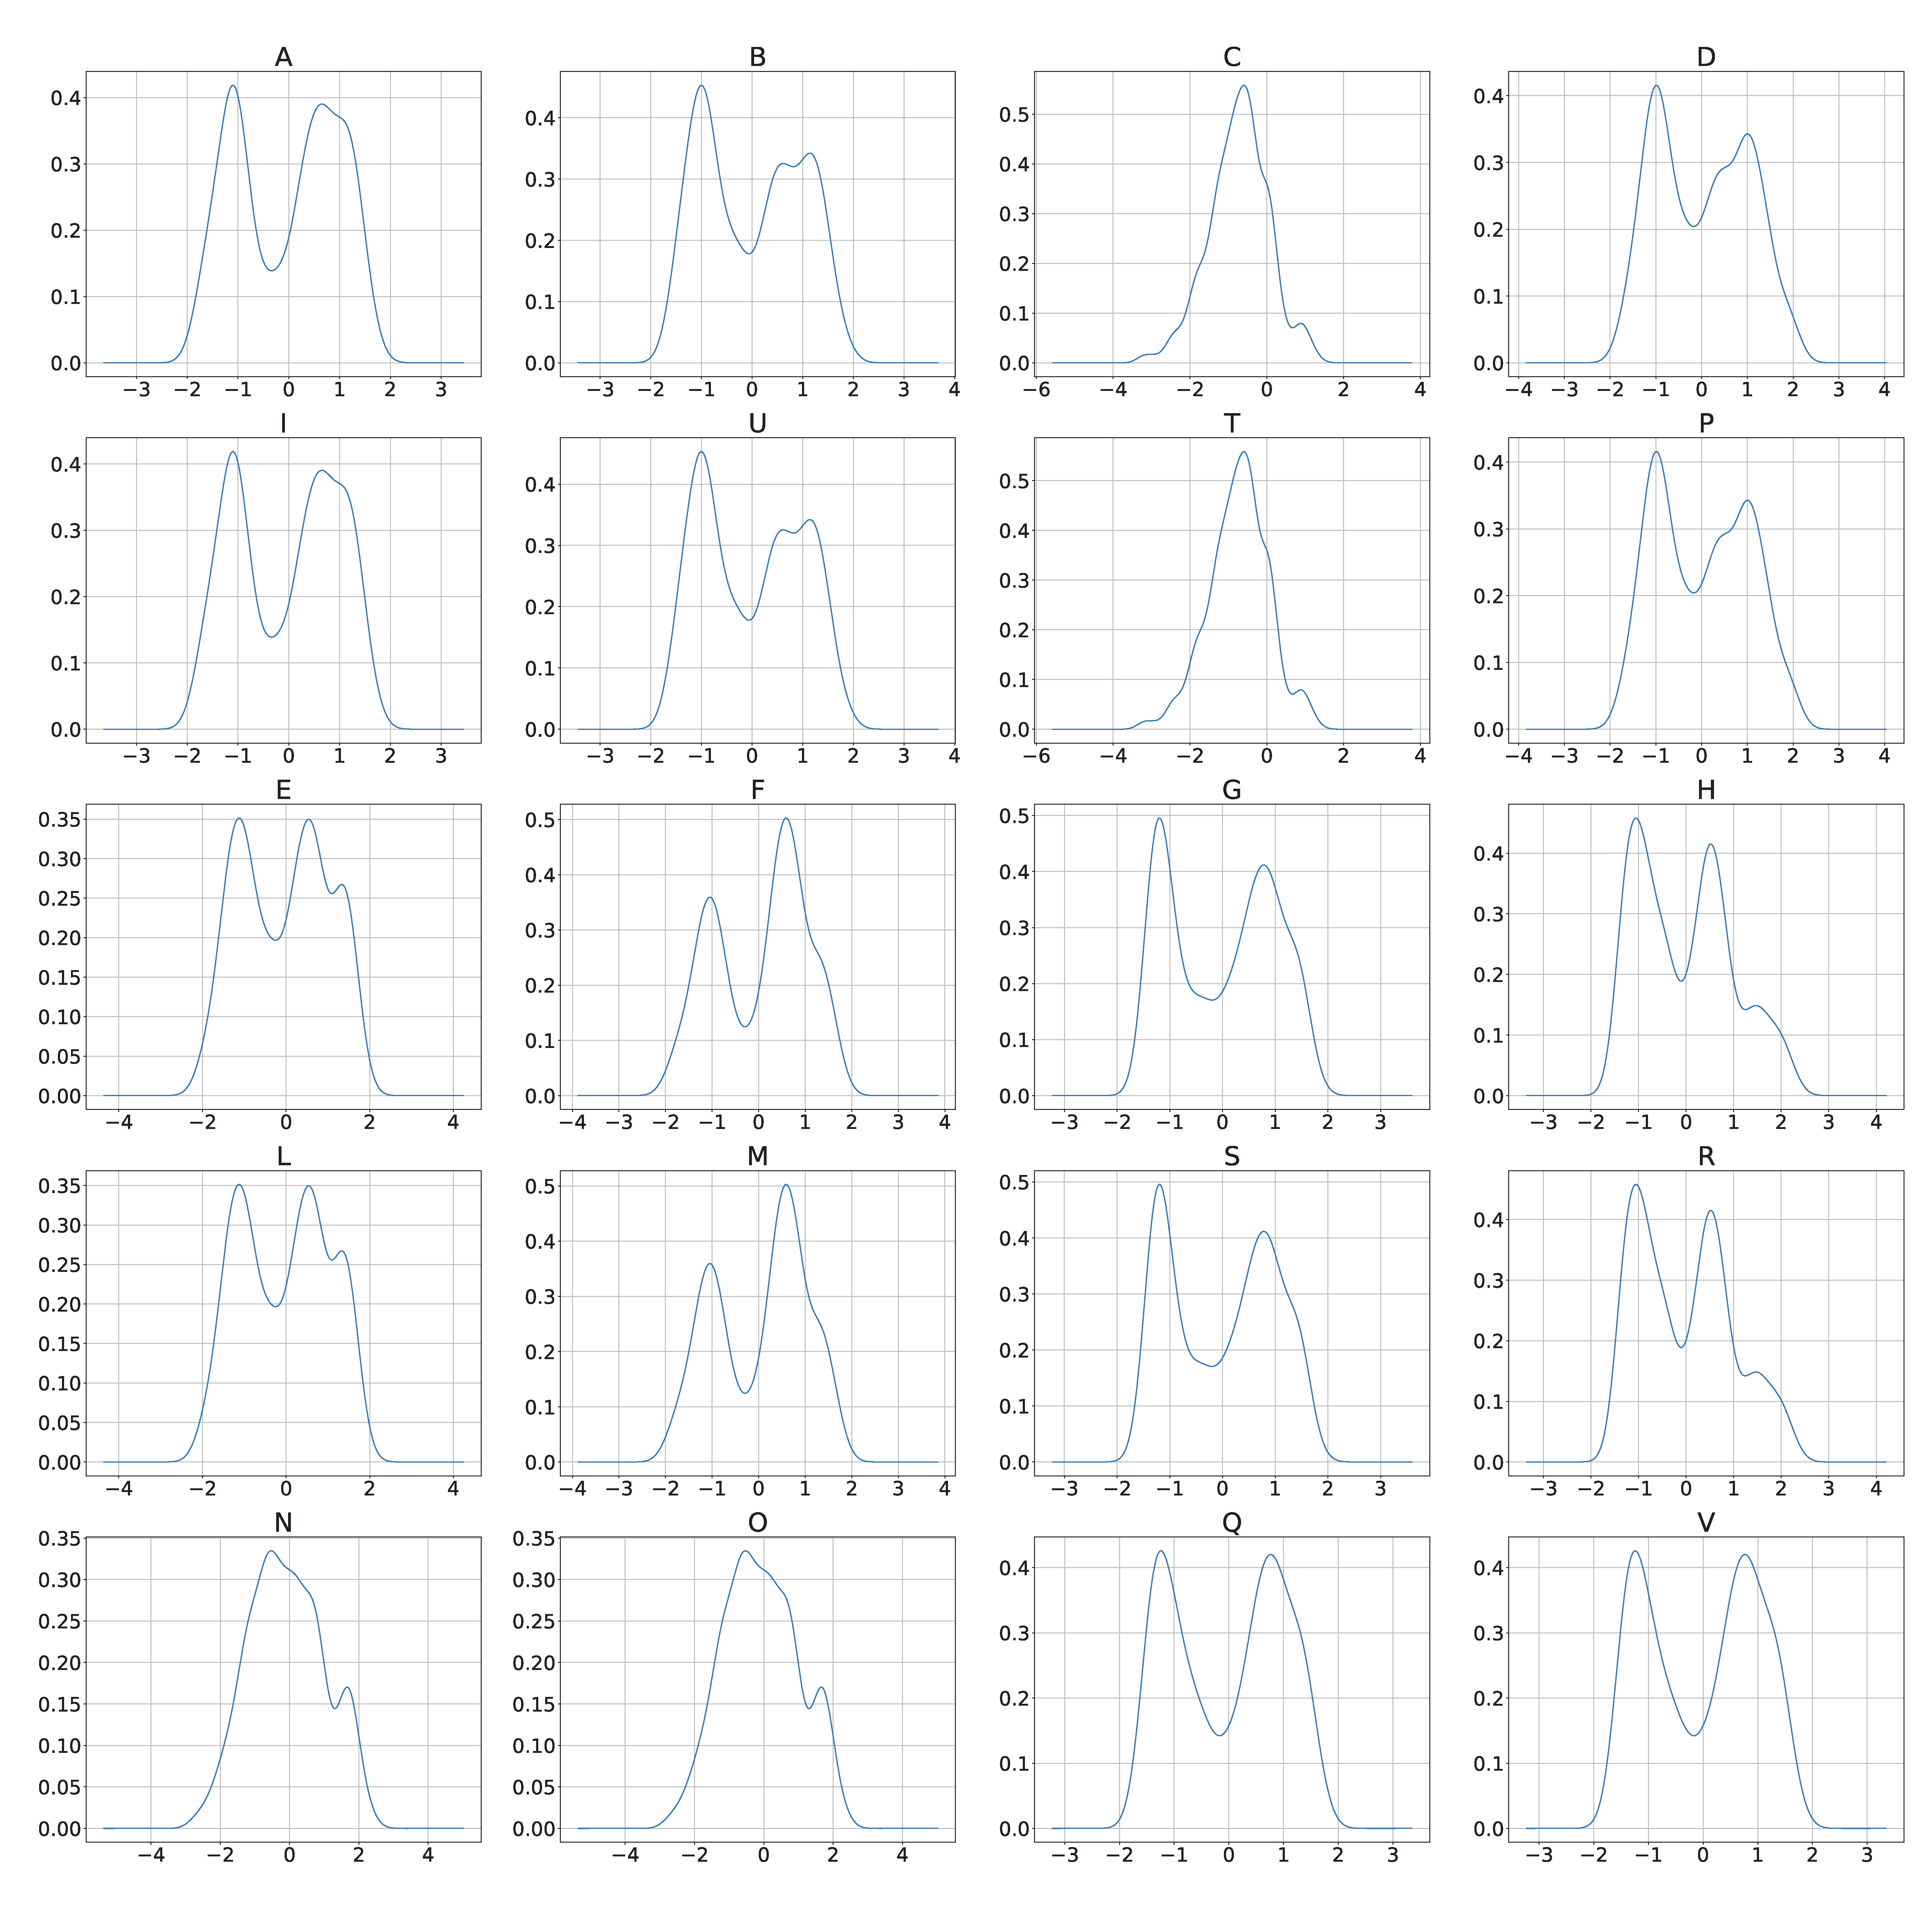
\includegraphics[scale = 0.16]{Images/preprocessing_phase/distributions_2.eps}
    \caption{Distributions of the features, excluded the one representing the id record and those relating to the target.}
    \label{fig:dis}
\end{figure}
\begin{figure}[H]
    \centering
    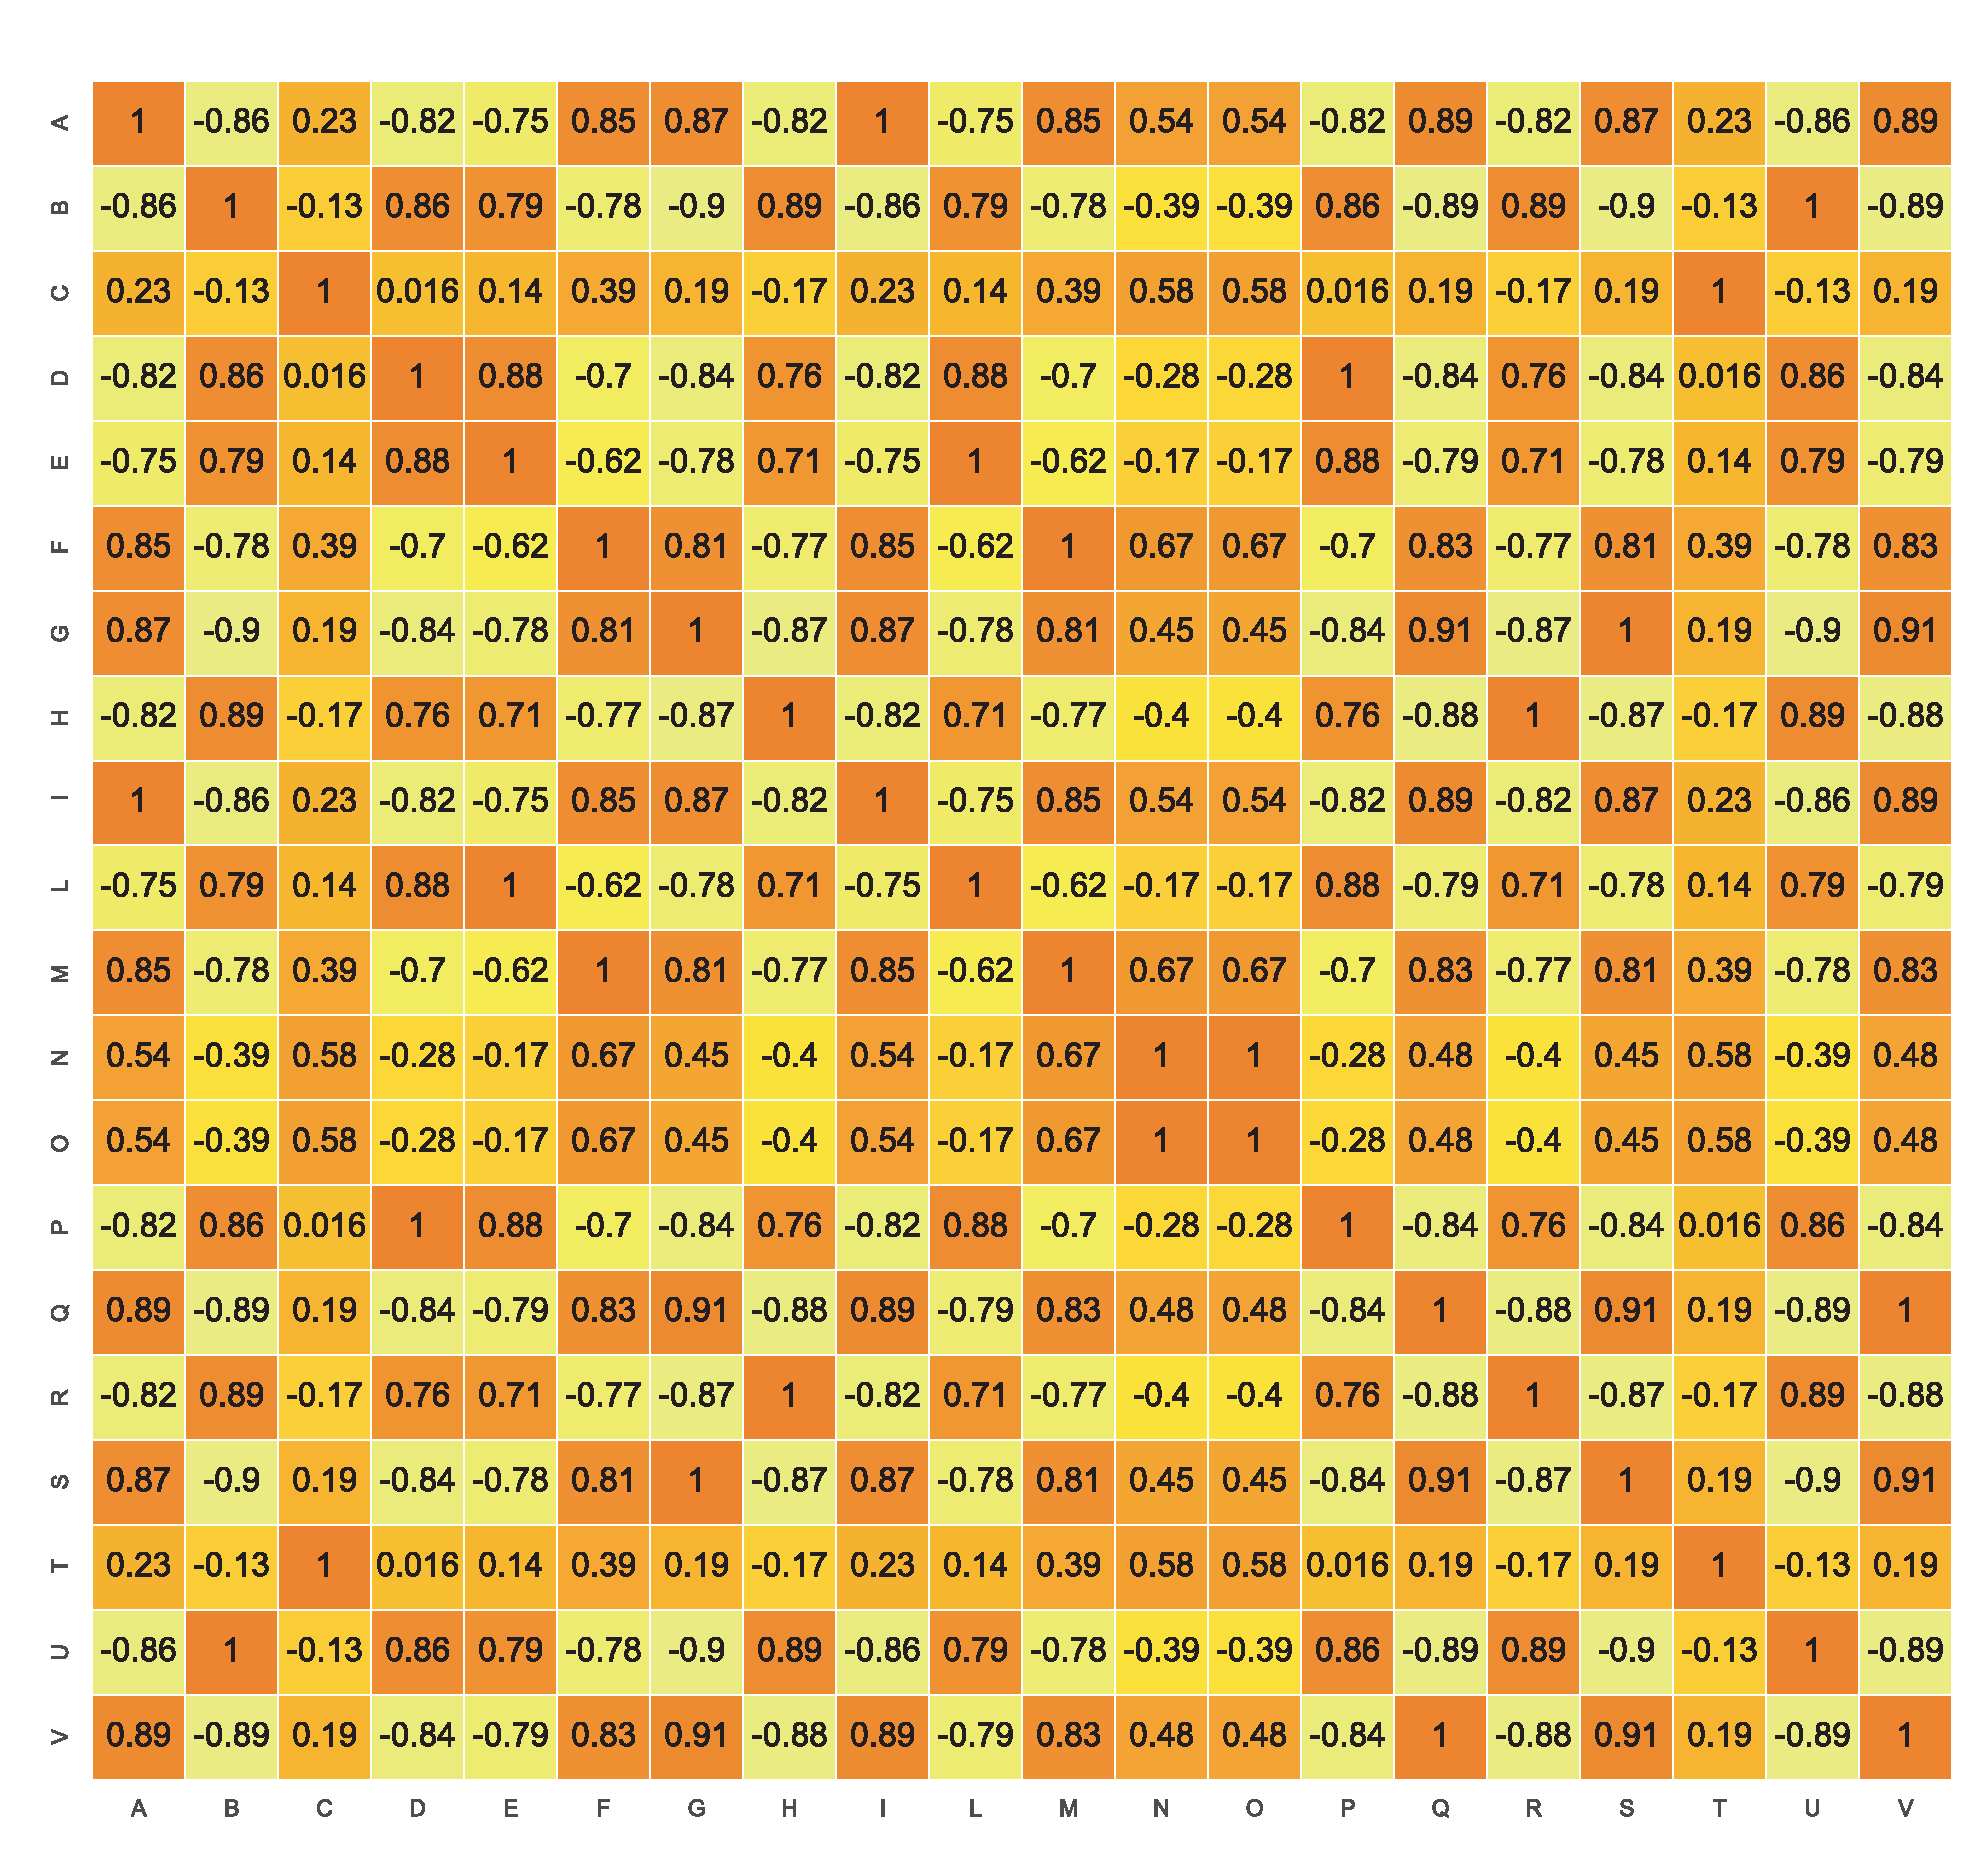
\includegraphics[scale = 0.5]{Images/preprocessing_phase/correlation_matrix_2.eps}
    \caption{Correlation matrix.}
    \label{fig:corr_mat}
\end{figure}
\end{appendices}


\end{document}
